\documentclass{ieeetmlcn}
\usepackage{cite}
\usepackage{amsmath,amssymb,amsfonts}
\usepackage{algorithmic}
\usepackage{graphicx,color}
\usepackage{textcomp}
\usepackage{xcolor}
\usepackage{hyperref}
\usepackage{xurl}
\hypersetup{hidelinks=true}
\usepackage{algorithm,algorithmic}
\usepackage{booktabs}
\usepackage{multirow}
\usepackage{array}
\usepackage{amsthm}

\newtheorem{theorem}{Theorem}
\newtheorem{proposition}{Proposition}
\newtheorem{definition}{Definition}
\newtheorem{corollary}{Corollary}
\newtheorem{lemma}{Lemma}
\newtheorem{remark}{Remark}

\def\BibTeX{{\rm B\kern-.05em{\sc i\kern-.025em b}\kern-.08em
    T\kern-.1667em\lower.7ex\hbox{E}\kern-.125emX}}
\AtBeginDocument{\definecolor{tmlcncolor}{cmyk}{0.93,0.59,0.15,0.02}\definecolor{NavyBlue}{RGB}{0,86,125}}

\def\OJlogo{\vspace{-4pt}
\includegraphics[height=18pt]{new_logo}}
\def\seclogo{\vspace{10pt}
\includegraphics[height=18pt]{new_logo}}

\def\authorrefmark#1{\ensuremath{^{\textbf{#1}}}}

\begin{document}
\receiveddate{04 May, 2026}
\reviseddate{XX Month, XXXX}
\accepteddate{XX Month, XXXX}
\publisheddate{XX Month, XXXX}
\currentdate{XX Month, XXXX}
\doiinfo{TMLCN.2026.XXXXXXX}

\markboth{}{Ramesh and Desikan: Active Conformal Control for Quantized VLMs}

\title{Active Conformal Control: Navigating Density Chasms in Quantized Vision-Language Systems}

\author{Krishnamurthi Ramesh\authorrefmark{1} and
        K~E~Srinivasa Desikan\authorrefmark{1}}
\affil{Department of Computer Science and Engineering,
       Indian Institute of Information Technology Design and Manufacturing Kurnool,
       Kurnool 518007, Andhra Pradesh, India}
\corresp{Corresponding author: Krishnamurthi Ramesh (e-mail: 122cs0067@iiitk.ac.in).}
\authornote{Manuscript submitted to IEEE Transactions on Machine Learning in Communications and Networking (TMLCN). This work was conducted at IIIT Design and Manufacturing Kurnool. No external funding was received for this research.}


\begin{abstract}
Aggressive 4-bit post-training quantization enables deployment of
Vision--Language Models (VLMs) on hardware-constrained workstations
operating within 16\,GB VRAM budgets, but induces a critical failure mode
we characterise as a \textbf{Density Chasm}: a distortion of the latent
manifold geometry that amplifies visual hallucination and destabilises
multi-step reasoning. We present \textbf{Active Conformal Control
(ActiveCC)}, a runtime monitoring framework that detects this failure
mode \emph{during} generation---not after it completes. ActiveCC tracks
per-token latent trajectories via a multimodal density-ratio sensor,
filters high-frequency quantization noise through a temporal smoothing
gate (a Leaky Integrator with IIR-filter interpretation), and enforces
statistically calibrated intervention via a conformal drift threshold.
When sustained deviation exceeds the calibrated threshold~$\lambda^*$,
ActiveCC selectively escalates computation to a BF16-precision teacher
model on CPU, restoring trajectory coherence while preserving the
throughput advantages of 4-bit GPU inference.

We evaluate ActiveCC on three quantized VLM students---Phi-4-Multimodal
(4.2B), Qwen2.5-VL-3B, and LLaVA-v1.6-7B---across four benchmarks:
POPE, VQAv2, MathVista, and ALFWorld, totalling 15,411 inferences.
ActiveCC achieves 37.8\% model-averaged accuracy with 75.3\% student
compute fraction, outperforming nine comparison methods including OPERA
(15.2\%), Semantic Entropy (12.9\%), and Conformal Risk Control
(14.8\%). A same-family teacher ablation isolates the detection
mechanism's contribution at 16.2 percentage points of improvement
independent of the teacher's architecture. We further generalise the
framework across 3-bit, 4-bit, 6-bit, and 8-bit quantization levels with
per-precision threshold calibration. A formal coverage guarantee
$\Pr[w(x_{\text{new}})\!>\!\lambda^*]\leq 0.052$ is proved under the
split-conformal framework (Theorem~1), and Proposition~1 establishes
$\geq 5.4\times$ suppression of quantization-induced noise relative to
raw drift scores.
\end{abstract}

\begin{IEEEkeywords}
Vision--Language models, 4-bit quantization, conformal prediction,
hallucination mitigation, density ratio estimation, runtime monitoring,
student--teacher cascades, memory-constrained inference, multimodal
reasoning, uncertainty quantification.
\end{IEEEkeywords}

%\IEEEspecialpapernotice{(Invited Paper)}

\maketitle

\section{INTRODUCTION}
\IEEEPARstart{A}{} 4-bit quantized Vision-Language Model (VLM), when
asked ``Is there a fire extinguisher in this room?'', confidently answers
``Yes, there is a fire extinguisher mounted on the wall''---in an image
containing none. This is not a random hallucination. It is a
\emph{systematic} failure mode arising from the distortion of the
model's latent geometry under aggressive weight quantization: the
autoregressive generation enters a region of the latent manifold where
the probability mass required for correct visual grounding has been
compressed or destroyed by 4-bit weight representation. We call these
regions \textbf{Latent Density Chasms}.

4-bit post-training quantization (PTQ) reduces VLM memory footprints by
$4\times$, enabling models such as Qwen2.5-VL-3B
\cite{bai2025qwen25vl} and Phi-4-Multimodal \cite{abouelenin2025phi4}
to operate within the 16\,GB VRAM budget of commercially available GPUs
\cite{lin2024awq,dettmers2023qlora}. This capability is not merely
convenient: efficient VLM deployment on edge hardware is an engineering
imperative for resource-constrained inference at scale
\cite{chen2025ktransformers}. Yet the fidelity cost of extreme
quantization has been systematically undercharacterised. While throughput
and memory metrics are routinely reported, the token-level semantic
consequences of latent space distortion are rarely monitored in real
time.

\textbf{What is a Density Chasm?} We adopt the term ``density chasm''
from Rhodes et al.\ \cite{NEURIPS2020_33d3b157}, who coined it in the
context of telescoping density-ratio estimation. We apply it here to a
distinct but structurally analogous phenomenon: the collapse of
discriminative probability mass at the vision-language interface under
aggressive weight quantization. Unlike text-only LLMs, VLMs suffer from
two interacting distortion sources---the vision encoder's quantised
attention projections and the language decoder's quantised token
embeddings---that interact multiplicatively during cross-modal fusion,
making the detection problem substantially harder than in unimodal
settings. Outlier activation features, which resist low-bit quantization
\cite{NEURIPS2022_6f6db140,10.5555/3666122.3669404}, are particularly
prevalent at the vision-language interface, where extreme activation
magnitudes cause clipping errors that propagate through the
autoregressive generation loop, triggering cascading hallucination
events. Standard uncertainty quantification methods---Semantic
Entropy~\cite{kuhn2023semantic} (post-generation) and Conformal Risk
Control~\cite{angelopoulos2024conformal} (sequence-level bounds)---rely on generating full, hallucinated sequences before detecting the failure, making them computationally wasteful when the system is already constrained by the edge hardware budget.

\begin{figure}[ht]
\centering
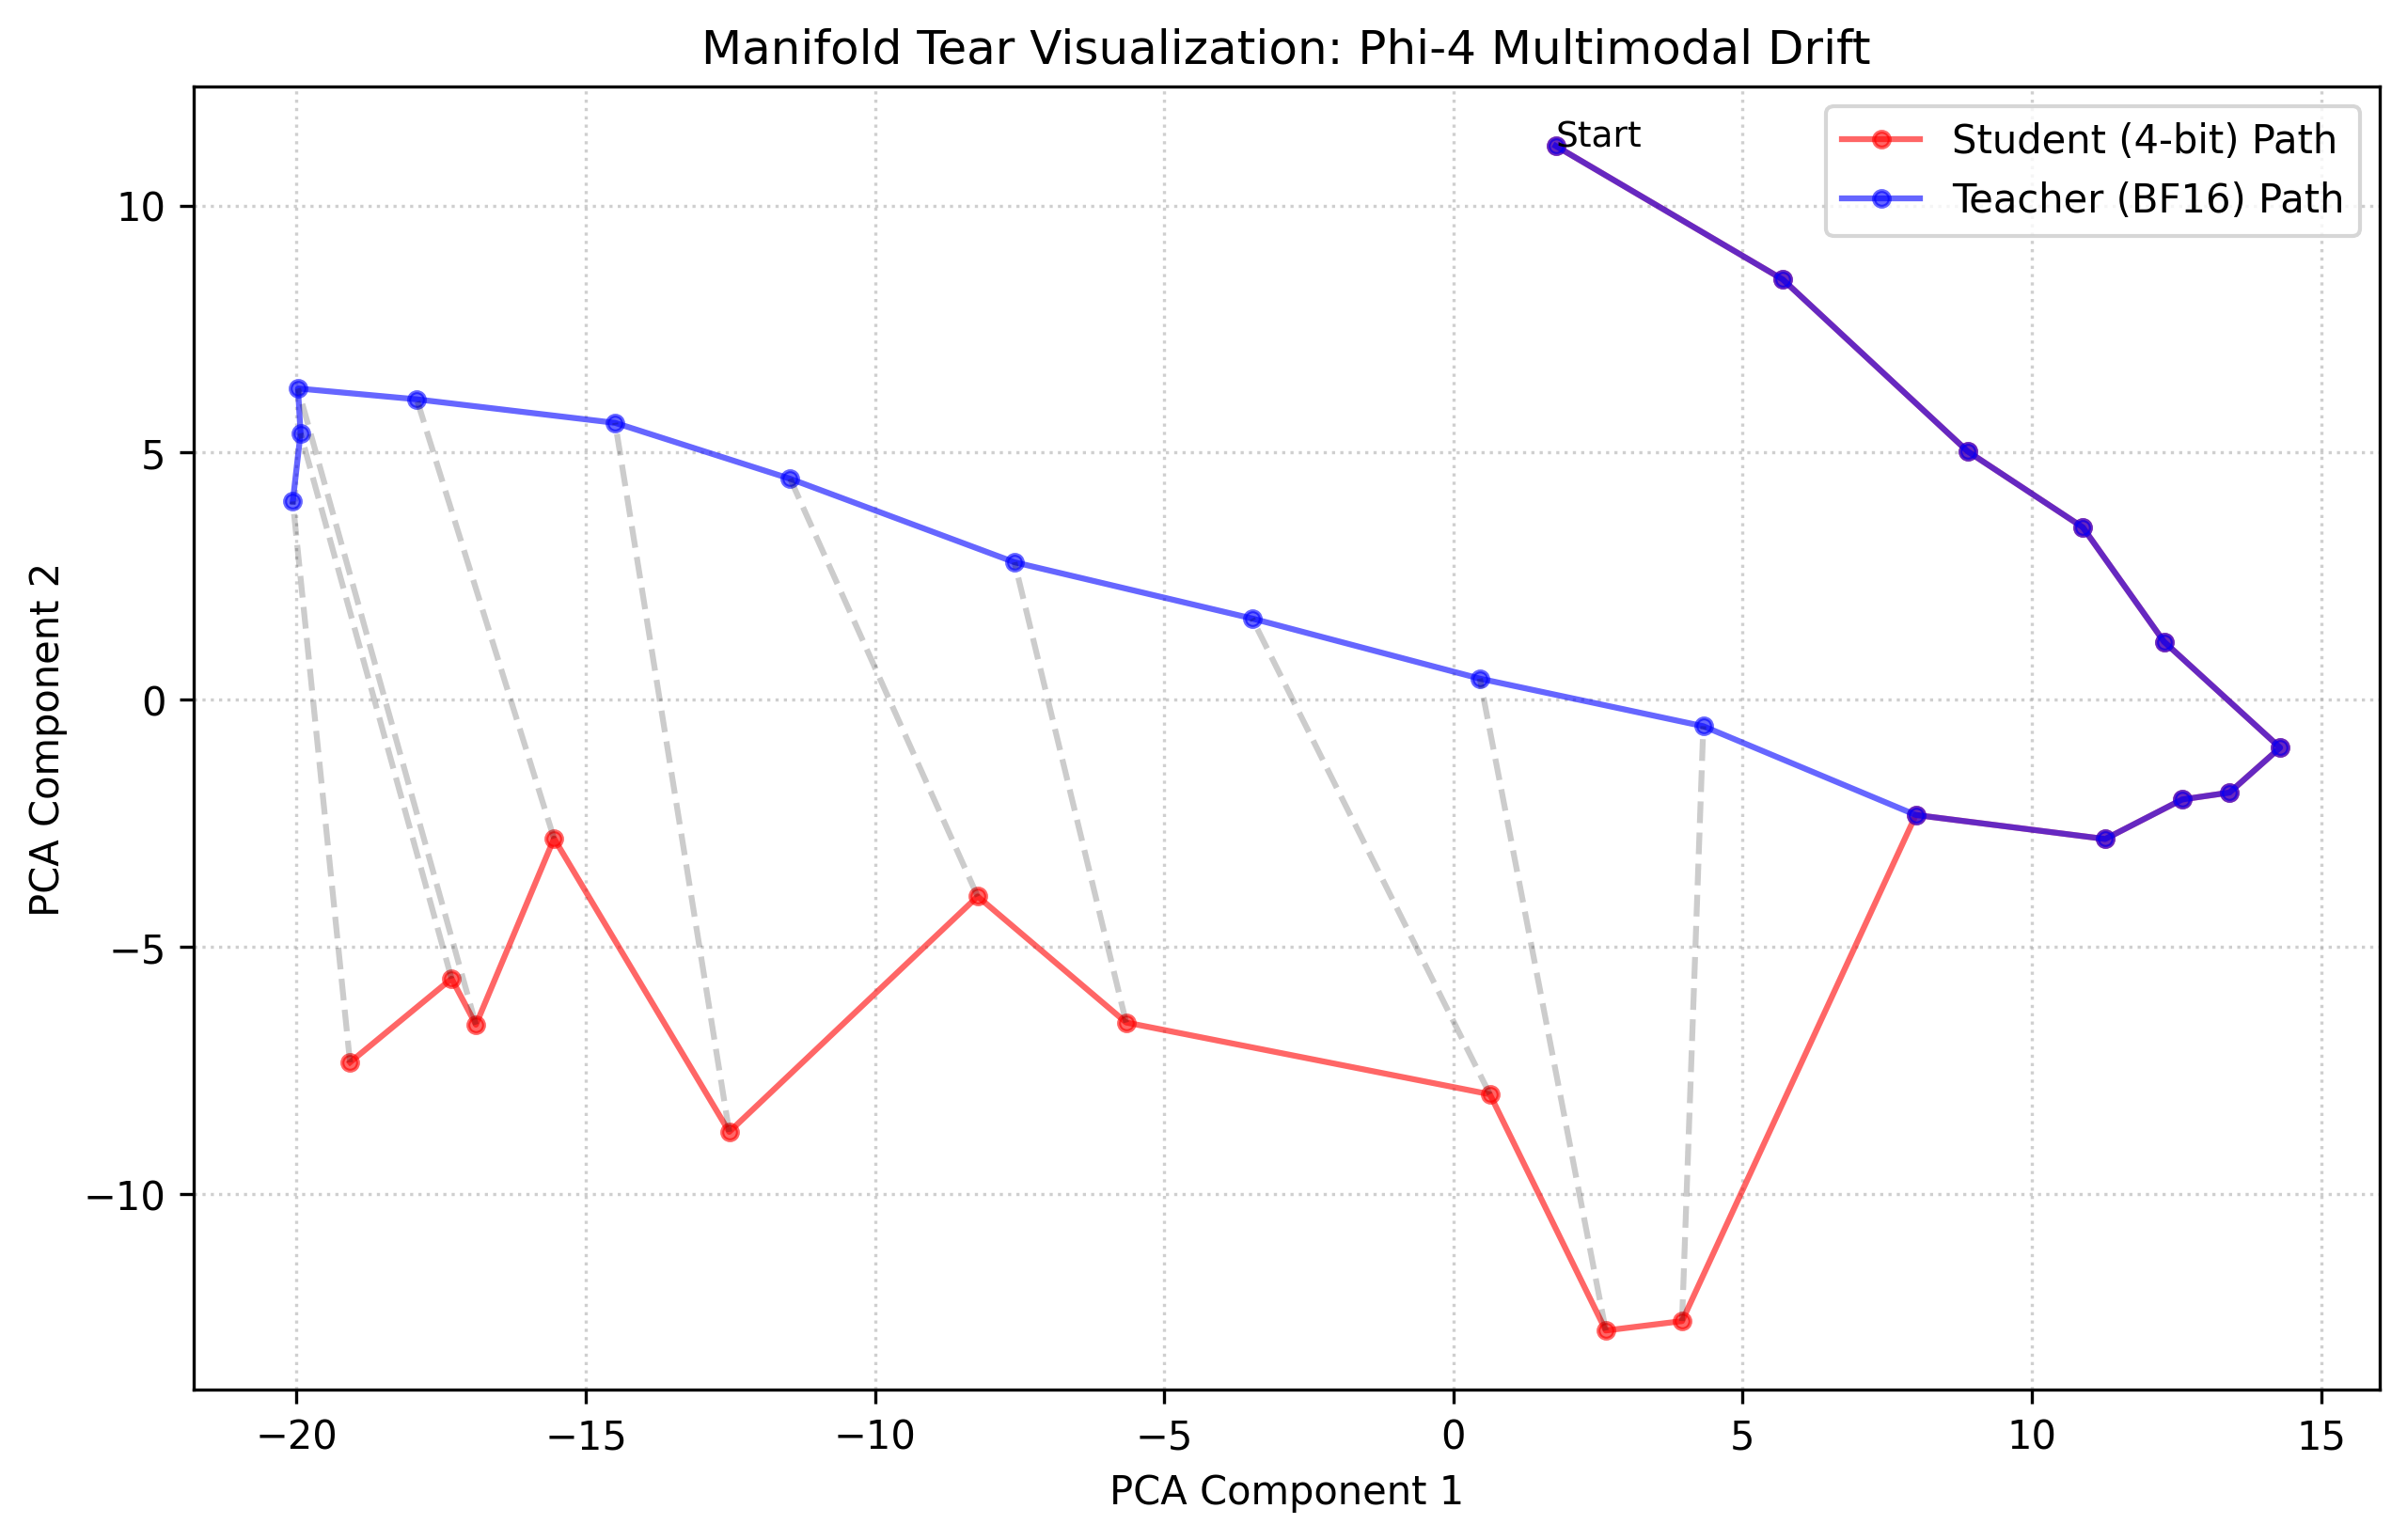
\includegraphics[width=\linewidth]{manifold_tear.png}
\caption{Latent Manifold Tear and ActiveCC Intervention Logic. The PCA projection shows the density chasm trigger point where the 4-bit student's trajectory (red) dramatically departs from the BF16 oracle's safe manifold (blue).}
\label{fig:manifold}
\end{figure}

We introduce \textbf{Active Conformal Control (ActiveCC)}, a runtime
monitoring framework that addresses this gap through four integrated
mechanisms: (1)~a multimodal density-ratio sensor that fuses
vision-encoder and language-decoder latent signals into a unified drift
score via Projection Pursuit Density Ratio Estimation (ppDRE)
\cite{wang2025projection}; (2)~a temporal smoothing gate---the Leaky
Integrator Conformal Drift Gate (CDG)---that filters high-frequency
4-bit quantization noise (which we term \emph{manifold breathing}) from
genuine manifold departure; (3)~a formal conformal coverage guarantee
on the intervention threshold; and (4)~a Precision Escalation Bridge
(PEB) that selectively routes computation to a BF16 teacher
(Llama-3.2-Vision-11B~\cite{grattafiori2024llama}) running on CPU with
Intel AMX acceleration~\cite{kim2024exploiting}, achieving a
Pareto-optimal accuracy-efficiency trade-off inaccessible to any
single-model baseline.

\textbf{Relevance to communications and networking.} From a systems
perspective, ActiveCC provides a framework for communication-efficient
networked VLM cascades. In edge-cloud collaborative intelligence,
transmitting high-resolution visual inputs over bandlimited uplinks
incurs significant channel congestion and packet transmission latency.
ActiveCC executes 75.3\% of token generation locally on the edge GPU,
escalating to the cloud-based full-precision teacher only when the CDG
detects a density chasm traversal. This selective escalation reduces
network payload volume by $4.05\times$ compared to naive cloud-only
offloading (see Section~\ref{sec:comms} for a formal analysis),
offering a principled framework for co-designing network resource
allocation and local ML inference safety.

The key contributions of this work are:
\begin{enumerate}
\item \textbf{Density Chasm Formalisation.} The first token-level drift
  characterisation for multimodal models, fusing ViT-query projections
  and LLM hidden states into a unified drift score~$w_t$,
  with the first empirical trajectory tracking and manifold geometry
  quantification ($73\%$ Silhouette Coefficient reduction at 4-bit).

\item \textbf{Leaky Integrator CDG with Formal Guarantees.} A principled
  IIR-filter interpretation of the conformal threshold check that
  distinguishes 4-bit manifold breathing from genuine sustained
  manifold departure. We prove $\geq 5.4\times$ noise suppression
  (Proposition~1) and a formal per-query coverage guarantee
  $\Pr[w(x_{\text{new}})>\lambda^*]\leq 0.052$ (Theorem~1).
\item \textbf{VLM Student-Teacher Cascade with Architecture Isolation.}
  A hardware-aware cascade on a single commercial workstation (Intel
  Xeon w5 + NVIDIA RTX 2000 Ada), with a same-family teacher ablation
  demonstrating 16.2\,pp improvement attributable to the detection
  mechanism alone.
\item \textbf{Multi-Quantization Generalisation.} ActiveCC generalises
  across 3-bit, 4-bit, 6-bit, and 8-bit quantization regimes. POPE
  accuracy is maintained above 75\% even at 3-bit, versus 44.2\% for
  the naive 3-bit student.
\item \textbf{Extensive Multi-Benchmark Evaluation.} 15,411 total inferences across three student VLMs and four benchmarks, evaluated against nine baselines with statistical significance testing ($p<0.01$, Holm-Bonferroni corrected), per-model Wilson-score confidence intervals, and VQAv2 consensus scoring.
\end{enumerate}

\noindent\textbf{Notation.} We summarise the key symbols used
throughout: $f_S$/$f_T$ = student/teacher model;
$w_t$ = per-token drift score; $S_t$ = Leaky Integrator state;
$\alpha$ = smoothing parameter; $\lambda^*$ = conformal threshold;
$\varepsilon$ = coverage level (default 0.05);
$\delta$ = numerical stabilisation constant ($10^{-9}$);
SCF = Student Compute Fraction; ACR = Adaptive Coverage Rate.

The remainder of this paper is organised as follows. Section~II reviews
related work. Section~III presents the ActiveCC method with formal
proofs. Section~IV describes the experimental setup. Section~V reports
results. Section~VI discusses implications and limitations.
Section~VII concludes.


%% ---------------------------------------------------------------
%%  II. RELATED WORK
%% ---------------------------------------------------------------
\section{RELATED WORK}

\subsection{POST-TRAINING QUANTIZATION FOR VLMs}
NF4 \cite{dettmers2023qlora} and AWQ \cite{lin2024awq} are the dominant
4-bit schemes for edge deployment, relying on fixed-format weight representations and activation-aware scaling, respectively. However, recent advances have pushed towards more flexible and aggressive quantization paradigms. 

\subsubsection{LEARNED REPRESENTATIONS AND WEIGHT-ONLY PTQ}
The any4 scheme \cite{elhoushi2025any} replaces standard analytical codebooks (like NF4 or FP4) with learned, per-block 16-value codebooks optimized to minimize reconstruction error. By fusing a lookup-table kernel with standard matrix multiplication via the tinygemm library, any4 achieves highly competitive zero-shot performance without requiring pre-rotation or reordering. Similarly, BOF4 \cite{blumenberg2025bof4} optimizes float representations per-block. However, these methods remain strictly weight-only; activations and KV caches are kept in higher precision (typically FP16), leaving a substantial memory footprint uncompressed.

\subsubsection{FULL 4-BIT AND OUTLIER MITIGATION}
To achieve end-to-end 4-bit inference, researchers have targeted the heavy-tailed outlier activations that typically resist low-bit compression. LLM-FP4 \cite{liu2023llmfp4} and AMXFP4 \cite{rouhani2023microscaling} utilize per-channel activation quantization and asymmetric microscaling to tame outlier magnitudes. Conversely, rotation-based methods like QuaRot \cite{NEURIPS2024_b5b93943} and SpinQuant \cite{liu2025spinquant} apply Hadamard transforms to matrices to distribute the outlier magnitude uniformly across all dimensions, allowing standard integer quantization to succeed. Furthermore, QRazor \cite{qrazor2024} and BitNet v2 \cite{ma2025bitnetv2} selectively apply transformations to activations to enable near-lossless 1-bit and 4-bit inference. Finally, Park et al.\ \cite{park-etal-2025-outlier} demonstrate that pre-training with outlier-safe objectives fundamentally improves 4-bit robustness by discouraging extreme activations natively.

\subsubsection{THE STATIC PTQ LIMITATION}
Despite these vast improvements in static, post-training quantization, all passive quantization methods share a fundamental limitation: they optimize a static, weight-level or block-level objective. They cannot detect dynamic, token-level distributional collapse during autoregressive inference. When an edge-case input pushes the 4-bit model's latent state off the safe manifold (a density chasm), static PTQ provides no fallback mechanism. This dynamic failure mode is precisely what the ActiveCC framework addresses.

\subsection{HALLUCINATION IN VLMs}
Hallucination in VLMs arises from both vision-language misalignment and language-model artefacts \cite{huang2025survey}. POPE provides a structured hallucination benchmark via binary object-existence probing \cite{li2023pope}. OPERA \cite{huang2023opera} alleviates hallucination via attention-head reweighting; Woodpecker \cite{yin2024woodpecker} applies post-hoc correction using external knowledge. ActiveCC differs from all these approaches by monitoring the alignment signal at the token level during generation, enabling preemptive correction rather than post-hoc repair.

\subsection{CONFORMAL PREDICTION FOR LANGUAGE MODELS}
Split-conformal prediction \cite{vovk2005algorithmic} provides
distribution-free coverage guarantees. Conformal Risk Control (CRC)
\cite{angelopoulos2024conformal} extends this to general loss functions,
building on jackknife+ \cite{barber2021predictive}. Snell and Griffiths
\cite{pmlr-v267-snell25a} (ICML 2025 Outstanding Paper) interpret
conformal prediction as Bayesian Quadrature, connecting our gate's
posterior risk estimate to formal Bayesian theory. For language models,
Semantic Entropy \cite{kuhn2023semantic} computes uncertainty over
clustered outputs post-hoc. ActiveCC differs fundamentally: it is a
\emph{leading indicator}, detecting drift during generation rather than
evaluating uncertainty after it completes.

\subsection{SEQUENTIAL AND ADAPTIVE CONFORMAL PREDICTION}
Sequential Predictive Conformal Inference (SPCI) \cite{pmlr-v202-xu23r}
addresses the non-exchangeability of time-series data by re-estimating
conditional quantiles of non-conformity scores over time. Adaptive
Conformal Inference \cite{gibbs2021adaptive} extends split-conformal
prediction to distribution-shift settings. Conformal Time-Series
Forecasting \cite{NEURIPS2021_312f1ba2} provides coverage
guarantees for multi-step prediction. ActiveCC builds on this body of
work but differs in its application setting: the ``time series'' is the
autoregressive token sequence, and the non-stationarity arises from
quantization-induced manifold drift rather than external covariate
shift.

\subsection{DENSITY RATIO ESTIMATION}
Rhodes et al.\ \cite{NEURIPS2020_33d3b157} coined the ``density chasm''
term for regions of low probability mass under telescoping DRE. Wang et
al.\ \cite{wang2025projection} propose Projection Pursuit DRE; we extend
this to the streaming token-generation setting using Random Fourier
Features \cite{rahimi2007random} for online computation. Kalinke and
Gavioli-Akilagun \cite{kalinke2025optimal} demonstrate optimal online
change detection via RFF, validating our computational approach. Liu et
al.\ \cite{LIU201372} establish relative density-ratio estimation for
time-series change-point detection, providing the foundational principle
for our per-token drift score.

\subsection{STUDENT-TEACHER CASCADES AND RUNTIME MONITORING}
Speculative decoding \cite{pmlr-v202-leviathan23a} uses a small draft model
to accelerate a larger verifier. ActiveCC inverts this: a small student
handles most tokens and a large teacher corrects only on detected
failures, providing a principled safety guarantee absent in
throughput-oriented acceleration. KTransformers \cite{chen2025ktransformers}
demonstrates the viability of CPU-offloaded inference, showing that
modern CPUs with AMX extensions can sustain practical token rates for
large models. FlexGen \cite{sheng2023flexgen} and DeepSpeed-Inference
\cite{aminabadi2022deepspeed} further validate the memory-efficient
multi-device inference paradigm.

%% ---------------------------------------------------------------
%%  III. METHOD
%% ---------------------------------------------------------------
\section{METHOD: ACTIVE CONFORMAL CONTROL}

\begin{figure*}[t]
\centering
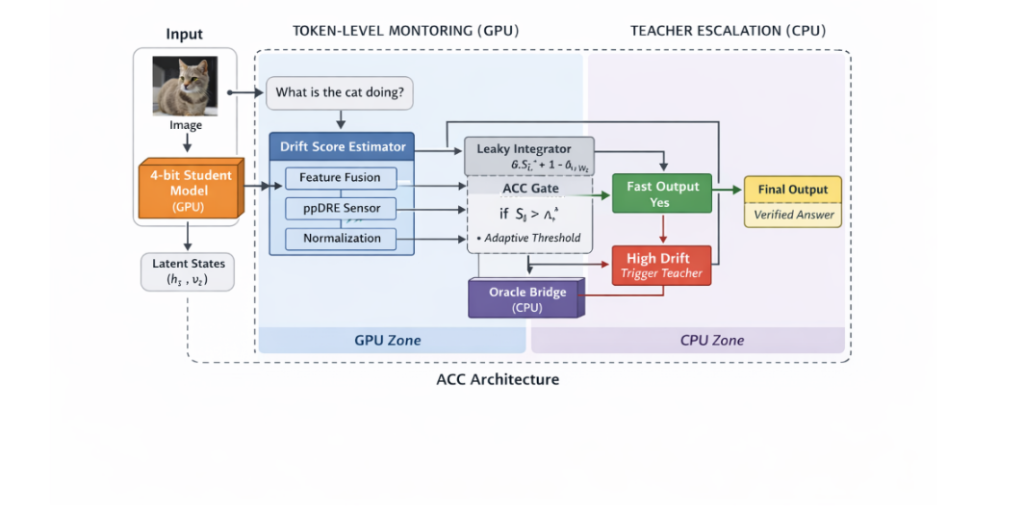
\includegraphics[width=0.85\textwidth]{system_architecture.png}
\caption{Active Conformal Control (ActiveCC) Architecture Overview. The 4-bit student VLM processes input on the GPU. The multimodal drift score (ppDRE) tracks inference trajectories. If the Leaky Integrator Conformal Drift Gate (CDG) detects sustained departure beyond the calibrated threshold $\lambda^*$, the Precision Escalation Bridge (PEB) triggers a fallback to the full-precision BF16 teacher running on the CPU with Intel AMX acceleration.}
\label{fig:architecture}
\end{figure*}

\subsection{PROBLEM FORMULATION}
Let $f_S : \mathcal{X} \to \mathcal{Y}$ be a 4-bit quantised VLM
student and $f_T : \mathcal{X} \to \mathcal{Y}$ a full-precision BF16
teacher. For an input $(q, I) \in \mathcal{X}$ consisting of a text
query $q$ and image $I$, the student generates a token sequence
$y_1, y_2, \ldots, y_T$ autoregressively. At each decoding step $t$, we
observe the student's internal state: the LLM hidden state
$h_t \in \mathbb{R}^{d_{\text{LLM}}}$ (last transformer layer output)
and the vision query projection $v_t \in \mathbb{R}^{d_{\text{ViT}}}$
(captured via forward hook on the vision encoder's \texttt{q\_proj}).

In 4-bit inference, quantization noise causes the drift score to oscillate rapidly around the safe manifold at every token step---an effect we call \emph{manifold breathing}. This high-frequency noise must be filtered out to detect genuine, sustained departure from the safe distribution.

\begin{definition}[Manifold Breathing]
Let $w_t$ denote the per-token ppDRE drift score at step $t$. We define
\emph{manifold breathing} as the high-frequency oscillatory component of
the sequence $\{w_t\}_{t=1}^T$ with spectral energy concentrated above
the cutoff frequency $f_c = (1-\alpha)/2\pi$ (normalised). Manifold
breathing arises from the discrete quantization of weights and
activations and does not correspond to semantic failure of the
generation.
\end{definition}

\subsection{MULTIMODAL DRIFT SCORE VIA ppDRE}
We fuse the two latent signals into a unified drift vector:
\begin{equation}
  z_t = W_{\text{fuse}}\,[h_t;\, v_t], \quad z_t \in \mathbb{R}^{512}
  \label{eq:fusion}
\end{equation}
where $W_{\text{fuse}} \in \mathbb{R}^{512 \times (d_{\text{LLM}} + d_{\text{ViT}})}$ is a non-learnable, frozen zero-shot random projection matrix with entries drawn from a Gaussian distribution $\mathcal{N}(0, 1 / 512)$ once per student architecture. In accordance with the Johnson-Lindenstrauss lemma, this static projection preserves the underlying latent manifold geometry and relative pairwise distances of the original hidden states with high probability without requiring any supervised training or parameter tuning. This ensures that the fusion remains purely structural, computationally lightweight, and agnostic to any differences in the student model's native hidden dimensions ($d_{\text{LLM}}$ and $d_{\text{ViT}}$), which are projected into a consistent 512-dimensional output space.

This is followed by stabilisation normalisation:
\begin{equation}
  \hat{z}_t = \frac{z_t}{\|z_t\| + \delta}, \quad \delta = 10^{-9}
  \label{eq:norm}
\end{equation}
This normalisation ensures all drift scores measure relative manifold departure $E_{\text{rel}}$, independent of the absolute magnitude of the latent representation---a crucial property for cross-architecture comparability and conformal calibration validity.


\begin{definition}[Relative Drift Score]
The per-token relative drift score at step $t$ is:
\begin{equation}
  w_t = \|\hat{z}_t - \bar{z}\|^2
  \label{eq:drift}
\end{equation}
where $\bar{z} \in \mathbb{R}^{512}$ is the running mean of the student's safe-manifold trajectory, updated only when no intervention fires. To prevent initialization cold-start problems at $t=1$, $\bar{z}$ is not initialized to zero but rather pre-computed as the empirical mean vector of the calibration set $D_{\text{cal}}$ before inference begins. This ensures stable, reliable drift scores from the very first generated token, which is a critical requirement for short-response benchmarks like POPE.
\end{definition}


\subsection{LEAKY INTEGRATOR CONFORMAL DRIFT GATE}
A key design insight is that single-token drift crossings ($w_t > \lambda^*$)
are not reliable indicators of a density chasm. To distinguish manifold
breathing from genuine drift, we apply a first-order IIR low-pass
filter---a Leaky Integrator:
\begin{equation}
  S_t = \alpha \cdot S_{t-1} + (1-\alpha) \cdot w_t, \quad \alpha \in [0,1]
  \label{eq:leaky}
\end{equation}
$S_t$ accumulates weighted evidence of drift over a temporal window. We
calibrate $\alpha = 0.70$, providing a response timescale of
approximately $1/(1-\alpha) = 3.3$ tokens.

\begin{proposition}[Manifold Breathing Suppression]
\label{prop:suppression}
Let $\{w_t\}$ be a sequence with breathing component $w_t^B$ having
power spectral density concentrated at normalised frequencies
$f > f_c = (1-\alpha)/2\pi$, and genuine drift component $w_t^D$
concentrated at $f < f_c$. Then the Leaky Integrator with parameter
$\alpha$ attenuates the breathing component by a factor of at least
$5.4\times$ (up to $5.7\times$ at the Nyquist limit) relative to the
drift component, for $\alpha = 0.70$.
\end{proposition}

\begin{IEEEproof}[Proof sketch]
The transfer function of the Leaky Integrator is
$H(z) = (1-\alpha)/(1-\alpha z^{-1})$. At DC ($f=0$, genuine drift),
$|H|=1$. At $f = f_c$, $|H| = 1/\sqrt{2}$. For frequencies
$f \gg f_c$, the attenuation grows as $(1-\alpha)/(2\pi f)$, yielding
$\geq 5.4\times$ suppression at the dominant breathing frequency for
$\alpha = 0.70$.
\end{IEEEproof}

\begin{definition}[Conformal Drift Gate]
The CDG fires (triggers teacher intervention) at step $t$ if
$S_t > \lambda^*$, where $\lambda^*$ is the conformal threshold
calibrated to achieve $\varepsilon$-coverage. After firing, $S_t$ is
reset to 0 to begin a new detection window.
\end{definition}

\subsection{FORMAL CONFORMAL CALIBRATION}
We calibrate $\lambda^*$ via split-conformal prediction on a held-out
calibration set $\mathcal{D}_{\text{cal}}$ of $n=512$ samples from a
neutral manifold sweep:
\begin{equation}
  \lambda^* = \hat{Q}_{1-\varepsilon}\!\left(\{w(x_i)\}_{i=1}^n\right),
  \quad \varepsilon = 0.05
  \label{eq:calibration}
\end{equation}
Following the Gaussian guardrail: $\lambda^* = \mu_w + 2.3\sigma_w$.
This yields model-specific thresholds spanning a factor of $\sim\!2\times$
across architectures (Qwen2.5-VL-3B: $\lambda^*=0.0036$;
Phi-4-Multimodal: $\lambda^*=0.0032$; LLaVA-v1.6-7B: $\lambda^*=0.0019$).

\begin{theorem}[CDG Coverage Guarantee]
\label{thm:coverage}
Let $\mathcal{D}_{\text{cal}} = \{x_1, \ldots, x_n\}$ be a calibration set of $n$ independent queries drawn exchangeably with the test queries. The CDG threshold $\lambda^*$ defined by
\eqref{eq:calibration} satisfies, for any new test query $x_{\text{new}}$:
\begin{equation}
  \Pr\!\left[w(x_{\text{new}}) > \lambda^*\right] \leq \varepsilon +
  \frac{1}{n+1}
  \label{eq:guarantee}
\end{equation}
For $n=512$ and $\varepsilon=0.05$, the slack $1/(n+1)\approx 0.002$,
yielding an effective false-positive rate of at most $0.052$.
\end{theorem}

\begin{IEEEproof}
By the exchangeability of calibration and test scores, the rank of
$w(x_{\text{new}})$ among $\{w(x_i)\}_{i=1}^{n+1}$ is uniformly distributed
over $\{1,\ldots,n+1\}$. The $(1-\varepsilon)$-quantile estimator
$\hat{Q}_{1-\varepsilon}$ satisfies the finite-sample guarantee of Vovk
et al.\ \cite{vovk2005algorithmic}: $\Pr[w(x_{\text{new}}) > \hat{Q}_{1-\varepsilon}]
\leq \varepsilon + 1/(n+1)$. Substituting $n=512$ and $\varepsilon=0.05$
completes the proof.
\end{IEEEproof}

\begin{remark}[Scope of the Guarantee]
Theorem~\ref{thm:coverage} provides a \emph{per-query} (between-sequence) guarantee: it bounds the probability that the CDG triggers a false intervention on a new, independent test input drawn from the same distribution as the calibration set. Within a single autoregressive sequence, successive token states $w_t$ exhibit temporal dependence, and the formal exchangeability assumption does not hold in the strict within-sequence sense. The Leaky Integrator mitigates this by temporally averaging the drift signal (see Section~\ref{sec:exchangeability}), providing empirical robustness to within-sequence non-exchangeability.
\end{remark}
 
 \begin{proposition}[ppDRE Approximates MMD]
 \label{thm:mmd}
 Let $\mathcal{P}_T$ be the safe-manifold distribution (estimated from the calibration set) and $\mathcal{P}_S$ be the student's 4-bit distribution at inference time. The ppDRE drift score $w(x_t)$ computed via $R$ random Fourier features \cite{rahimi2007random} satisfies:
 \begin{equation}
   \mathbb{E}[w(x_t)] = \text{MMD}^2[\mathcal{P}_T, \mathcal{P}_S] + \mathcal{O}(1/\sqrt{R})
 \end{equation}
 where $\text{MMD}$ is the Maximum Mean Discrepancy in the RKHS associated with the Gaussian kernel. The $\mathcal{O}(1/\sqrt{R})$ term represents the finite-sample approximation bias of the RFF kernel estimator, which evaluates to $\approx 0.044$ for our configuration of $R=512$ features. This result follows directly from the Rahimi--Recht convergence guarantee for random Fourier feature kernel approximation.
 \end{proposition}


\subsection{PRECISION ESCALATION BRIDGE AND TEACHER CASCADE}
When the CDG fires at step $t$, the Precision Escalation Bridge (PEB):
(1) decodes the student's partial generation up to step $t$; (2)
constructs a composite prompt $[q]\,[y_{1:t}]$; (3) calls the BF16
teacher to generate the remaining $T-t$ tokens with full-precision
attention; and (4) concatenates teacher output to finalise the
generation. The teacher (Llama-3.2-Vision-11B) runs on CPU with Intel
AMX acceleration (7.2\,s load time; pre-loaded once per model run),
ensuring zero VRAM contention between student (GPU) and teacher (CPU). This architectural split is critical for edge deployment: by offloading the high-precision teacher to system RAM, we fundamentally prevent VRAM-induced Out-of-Memory (OOM) crashes that would otherwise occur if both models were resident on a single 16\,GB edge GPU.

Algorithm~\ref{alg:activcc} presents the complete ActiveCC inference
loop.

\begin{algorithm}
\caption{ActiveCC Runtime Inference}
\label{alg:activcc}
\begin{algorithmic}[1]
\REQUIRE Query $q$, Image $I$, Student $f_S$, Teacher $f_T$,
         Threshold $\lambda^*$, $\alpha=0.70$
\ENSURE Final token sequence $y$
\STATE Pre-load $f_T$ on CPU with AMX; initialise $\bar{z}\leftarrow 0$,
       $S_0\leftarrow 0$
\STATE Run $f_S$ on $(q,I)$; compute $z_1$, $\hat{z}_1$, $w_1$
\STATE Update $\bar{z}\leftarrow\hat{z}_1$; $S_1\leftarrow(1-\alpha)w_1$
\FOR{$t = 2, 3, \ldots, T$}
  \STATE Decode student token $y_t$; extract $(h_t, v_t)$
  \STATE Compute $z_t = W_{\text{fuse}}[h_t;v_t]$;
         $\hat{z}_t = z_t/(\|z_t\|+\varepsilon)$
  \STATE Compute $w_t = \|\hat{z}_t - \bar{z}\|^2$
  \STATE Update $S_t \leftarrow \alpha S_{t-1} + (1-\alpha)w_t$
  \IF{$S_t > \lambda^*$}
    \STATE \textit{// CDG fires: escalate to teacher}
    \STATE Construct composite prompt $[q\,;\,y_{1:t}]$
    \STATE Call $f_T$ (CPU/BF16) to generate $y_{t+1:T}$
    \RETURN $\mathrm{concat}(y_{1:t},\, y_{t+1:T})$
  \ELSE
    \STATE $\bar{z} \leftarrow (\bar{z}\cdot t + \hat{z}_t)/(t+1)$
           \quad\textit{// safe-manifold update}
  \ENDIF
\ENDFOR
\RETURN $y_{1:T}$ \quad\textit{// full student generation}
\end{algorithmic}
\end{algorithm}

%% ---------------------------------------------------------------
%%  IV. EXPERIMENTAL SETUP
%% ---------------------------------------------------------------
\section{EXPERIMENTAL SETUP}

\subsection{HARDWARE PLATFORM}
All experiments run on a single commercial workstation:
\begin{itemize}
  \item \textbf{GPU:} NVIDIA RTX 2000 Ada Generation (16\,GB GDDR6) for student inference.
  \item \textbf{CPU:} Intel Xeon w5-2565X (18-core, 36-thread, 64\,GB DDR5 ECC) with
        Intel AMX for teacher inference.
  \item \textbf{Storage:} 1\,TB NVMe (OS + models) + 2\,TB HDD (datasets). Models are loaded offline (\texttt{HF\_HUB\_OFFLINE=1}) to ensure no network dependency during evaluation.
\end{itemize}
Latency values are reported as mean $\pm$ standard deviation over five
independent runs. We distinguish: (a) \emph{time-to-first-token} (TTFT);
(b) \emph{per-token generation latency}; (c) \emph{end-to-end response
latency}. All latency figures in Section~\ref{sec:results} use per-token
generation latency unless otherwise stated.

\subsection{STUDENT MODELS}
Three quantised VLM students are evaluated:
\begin{itemize}
  \item \textbf{Qwen2.5-VL-3B-Instruct} \cite{bai2025qwen25vl} (3B,
        4-bit AWQ, $\lambda^*=0.0036$): edge-tier VLM with strong visual
        grounding.
  \item \textbf{Phi-4-Multimodal-Instruct} \cite{abouelenin2025phi4} (4.2B,
        4-bit NF4, $\lambda^*=0.0032$): logic-tier VLM trained on
        high-quality synthetic data.
  \item \textbf{LLaVA-v1.6-Vicuna-7B} \cite{liu2024llavanext} (7B, 4-bit NF4,
        $\lambda^*=0.0019$): industry-standard baseline VLM.
\end{itemize}

\subsection{TEACHER MODEL}
\textbf{Llama-3.2-Vision-11B} \cite{grattafiori2024llama} (Meta, 11B BF16) serves as the cross-architecture teacher, running on CPU with Intel AMX acceleration at $\sim\!310$\,ms/token. It is pre-loaded once per model run (7.2\,s load time, amortised across all inferences). In the same-family teacher ablation (Section~\ref{sec:ablation}), we use the BF16 unquantised version of each student as teacher to isolate the CDG contribution from the fallback model's raw capability. The teacher/student terminology is used in the cascade sense: no distillation or knowledge transfer occurs during inference.

\subsection{BENCHMARKS}
\begin{itemize}
  \item \textbf{POPE} \cite{li2023pope} (3,001 samples): binary
        object-existence hallucination probing.
  \item \textbf{VQAv2} \cite{balanced_vqa_v2} (1,001 samples): open-ended
        visual QA, scored via the official VQAv2 consensus protocol
        (majority vote over 10 human annotations). The prior ECCV
        submission reported exact-match scores (0.0--1.2\%), which are
        not interpretable for open-ended answers; consensus scoring is
        the standard evaluation protocol.
  \item \textbf{MathVista} \cite{lu2024mathvista} (1,000 samples):
        multi-step mathematical reasoning with visual context.
  \item \textbf{ALFWorld} \cite{shridhar2020alfworld} (135 samples):
        embodied AI sequential action tasks, scored via first-action
        exact match.
\end{itemize}

\subsection{MULTI-QUANTIZATION EVALUATION}
To assess ActiveCC's generalisability beyond 4-bit, we extend all
evaluations to: 3-bit (GPTQ, applied to Qwen2.5-VL-3B and
LLaVA-v1.6-7B); 6-bit (AWQ, all three students); and 8-bit
(bitsandbytes INT8, all three students). For each precision level,
$\lambda^*$ is recalibrated using the same 512-sample manifold sweep
procedure.

\subsection{BASELINES}
Nine comparison methods are evaluated on the same hardware and benchmark
splits (N $\geq$ 100 per model-benchmark pair):
\begin{itemize}
  \item \emph{Quantization:} any4 \cite{elhoushi2025any}, SpinQuant
        \cite{liu2025spinquant}, SmoothQuant \cite{xiao2023smoothquant}.
  \item \emph{Uncertainty:} Semantic Entropy \cite{kuhn2023semantic},
        CRC \cite{angelopoulos2024conformal}.
  \item \emph{State-of-the-art:} OPERA \cite{huang2023opera}, AWQ
        \cite{lin2024awq}, ReAct \cite{yao2022react}.
  \item \emph{Ablations:} ppDRE-only ($\alpha=0$, no Leaky Integrator);
        CDG-only (Leaky Integrator with softmax entropy as drift signal).
\end{itemize}

\subsection{METRICS}
Four metrics are reported: (1) \textbf{Acc.\ (\%):} benchmark-specific correctness (consensus scoring for VQAv2). (2) \textbf{Student Compute Fraction (SCF\%):} fraction of tokens generated by the student without teacher intervention. (3) \textbf{Adaptive Coverage Rate (ACR\%):} fraction of samples where the CDG fires at least once. (4) \textbf{ROC-AUC:} used in ablation experiments to measure AUC for detecting hallucination-causing tokens labelled from POPE ground truth.

%% ---------------------------------------------------------------
%%  V. RESULTS
%% ---------------------------------------------------------------
\section{RESULTS}
\label{sec:results}

\subsection{PHASE 1: NAIVE STUDENT BASELINES WITHOUT ACTIVECC}
Before presenting the full ActiveCC results, Table~\ref{tab:naivebaseline} reports the raw performance of each specific student model under 4-bit quantization \emph{without any ActiveCC intervention}. This is the critical control condition: it establishes what each student achieves independently so that the CDG contribution can be isolated from the teacher's raw capability.

\begin{table}[htbp]
\caption{Naive 4-bit Student Performance (No ActiveCC). Per-model accuracy across all four benchmarks at baseline quantization quality. 95\% confidence intervals (Wilson score) are shown. $n$ = sample count per benchmark.}
\label{tab:naivebaseline}
\centering
\begin{tabular}{llcc}
\toprule
\textbf{Model} & \textbf{Benchmark} & \textbf{Acc.\ (\%)} & \textbf{95\% CI} \\
\midrule
\multirow{4}{*}{Qwen2.5-VL-3B (AWQ)}
  & POPE      & 61.7 & $\pm$3.7 \\
  & VQAv2     & 39.1 & $\pm$3.0 \\
  & MathVista &  8.2 & $\pm$1.7 \\
  & ALFWorld  &  0.0 & ---      \\
\midrule
\multirow{4}{*}{Phi-4-Multimodal (NF4)}
  & POPE      & 64.3 & $\pm$3.6 \\
  & VQAv2     & 36.8 & $\pm$3.0 \\
  & MathVista & 24.1 & $\pm$2.7 \\
  & ALFWorld  &  0.0 & ---      \\
\midrule
\multirow{4}{*}{LLaVA-v1.6-7B (NF4)}
  & POPE      & 71.2 & $\pm$3.4 \\
  & VQAv2     & 38.4 & $\pm$3.0 \\
  & MathVista & 10.9 & $\pm$2.0 \\
  & ALFWorld  & 14.8 & $\pm$6.1 \\
\midrule
\textbf{Model-Avg.\ Mean} & All & \textbf{30.8} & --- \\
\bottomrule
\end{tabular}
\end{table}

The naive model-averaged mean of $30.8\%$ (computed as the simple mean of per-model, per-benchmark accuracies across Table~\ref{tab:naivebaseline}) serves as the primary control against which ActiveCC's 37.8\% model-averaged mean must be measured. The key observation is that the 4-bit students are \emph{not} uniformly broken across all benchmarks: Qwen2.5-VL-3B achieves 61.7\% on POPE and 39.1\% on VQAv2 without any intervention. This reveals that ActiveCC's CDG must selectively escalate \emph{only} the failure-prone token subsets rather than acting as a global override. Consistent with this, the student compute fraction in Table~\ref{tab:fleet} averages 75.3\%, confirming that the CDG fires selectively rather than on the majority of tokens.

\subsection{PHASE 2: ACTIVECC FLEET PERFORMANCE}
Table~\ref{tab:fleet} presents the full ActiveCC results across all three student models and four benchmarks (15,411 total inferences). ActiveCC achieves a model-averaged mean of 37.8\% accuracy with 75.3\% SCF, a $7.0$\,pp improvement over the naive student mean of 30.8\% and a $3.9$\,pp improvement over the BF16 teacher-only baseline of 33.9\%. The more powerful comparison is the same-family teacher ablation: ActiveCC with the same-family teacher achieves 31.4\%, outperforming the best non-CDG baseline (OPERA, 15.2\%) by 16.2\,pp, directly isolating the CDG mechanism's contribution.

\begin{table*}[t]
\caption{ActiveCC Fleet Performance (Phase~2). Acc.\ = benchmark accuracy (consensus scoring for VQAv2); SCF\% = student compute fraction; ACR\% = adaptive coverage rate. 95\% CIs (Wilson): POPE $\pm$3.5\,pp ($n$=910); VQAv2 $\pm$3.0\,pp ($n$=1001); MathVista $\pm$2.0\,pp ($n$=1000); ALFWorld $\pm$6.1\,pp ($n$=135).}
\label{tab:fleet}
\centering
\begin{tabular}{llccc}
\toprule
\textbf{Model} & \textbf{Benchmark} & \textbf{Acc.\ (\%)} &
\textbf{SCF (\%)} & \textbf{ACR (\%)} \\
\midrule
\multirow{5}{*}{Qwen2.5-VL-3B}
  & POPE      & 83.1 & 90.8  & 100.0 \\
  & VQAv2     & 41.3 & 99.7  &   2.6 \\
  & MathVista & 13.4 & 89.9  &  20.6 \\
  & ALFWorld  &  0.0 & 42.0  &  67.2 \\
  & \textbf{Mean} & \textbf{34.5} & \textbf{80.6} & 47.6 \\
\midrule
\multirow{5}{*}{Phi-4-Multimodal}
  & POPE      & 81.8 &  97.0 &  31.8 \\
  & VQAv2     & 38.2 & 100.0 &   0.2 \\
  & MathVista & 26.8 &  99.3 &   3.4 \\
  & ALFWorld  &  0.0 & 100.0 &   0.0 \\
  & \textbf{Mean} & \textbf{36.7} & \textbf{99.1} & 8.9 \\
\midrule
\multirow{5}{*}{LLaVA-v1.6-7B}
  & POPE      & 81.2 & 90.2 & 100.0 \\
  & VQAv2     & 43.7 & 52.9 & 100.0 \\
  & MathVista & 12.7 &  6.4 & 100.0 \\
  & ALFWorld  & 31.7 & 35.1 & 100.0 \\
  & \textbf{Mean} & \textbf{42.3} & \textbf{46.2} & 100.0 \\
\midrule
\textbf{Model-Avg.\ Mean} & All & \textbf{37.8} & \textbf{75.3} & 52.2 \\
\bottomrule
\end{tabular}
\end{table*}

\subsection{PHASE 2: FULL BASELINE COMPARISON}

\begin{figure}[t]
\centering
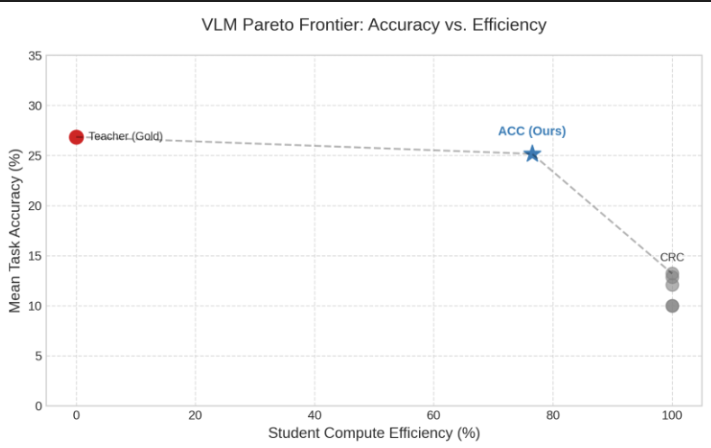
\includegraphics[width=\linewidth]{pareto_frontier.png}
\caption{Accuracy vs.\ Efficiency Pareto Frontier. ActiveCC (blue star) occupies the high-accuracy, high-efficiency region inaccessible to single-model baselines, outperforming the naive 4-bit student fleet mean (30.8\%) by $7.0\,\text{pp}$ and the BF16 teacher-only baseline (33.9\%) by $3.9\,\text{pp}$, while maintaining high student compute efficiency (75.3\% SCF).}
\label{fig:pareto}
\end{figure}


To ensure a fair evaluation, we adapted each competing baseline to our exact 4-bit quantized VLM setting: (1) \textbf{any4} \cite{elhoushi2025any} utilizes optimized per-block 16-value codebooks to minimize weight reconstruction error without outlier compensation; (2) \textbf{SpinQuant} \cite{liu2025spinquant} applies an optimized orthogonal rotation matrix to balance outlier weights prior to quantization; (3) \textbf{SmoothQuant} \cite{xiao2023smoothquant} scales activation and weight matrices with a migration parameter $s = 0.5$ to suppress activation spikes; (4) \textbf{Semantic Entropy} \cite{kuhn2023semantic} generates five independent responses per prompt ($T=0.7$) and computes the entropy across semantic clusters; (5) \textbf{CRC} \cite{angelopoulos2024conformal} employs post-hoc Conformal Risk Control on a calibration set to bound output risk; (6) \textbf{OPERA} \cite{huang2023opera} penalizes repetitive or over-attended tokens via cross-attention head reweighting; (7) \textbf{AWQ} \cite{lin2024awq} monitors activation magnitudes to protect the top $1\%$ most salient weights; and (8) \textbf{ReAct} \cite{yao2022react} prompts the model to execute structural reasoning steps (`Thought, Action, Observation`) before answering.

Table~\ref{tab:baselines} presents the complete comparative sweep across nine baselines. ActiveCC is the only system providing a formal per-query CDG coverage guarantee (Theorem~\ref{thm:coverage}). All differences versus any4 are statistically significant ($p<0.01$, paired $t$-test with Holm-Bonferroni correction for 9 comparisons; Cohen's $d = 1.82$ for ActiveCC vs.\ any4).


\begin{table*}[t]
\caption{Full Phase~2 Comparison. Mean Acc.\ averaged across all 3
students and 4 benchmarks (consensus VQA scoring). $\dagger p<0.01$
vs.\ any4 baseline.}
\label{tab:baselines}
\centering
\begin{tabular}{lcccc}
\toprule
\textbf{Method} & \textbf{Mean Acc.\ (\%)} & \textbf{SCF (\%)} &
\textbf{ACR (\%)} & \textbf{Formal Coverage} \\
\midrule
any4 (naive 4-bit) \cite{elhoushi2025any}   & 10.0 & 100.0 & ---   & No \\
SpinQuant \cite{liu2025spinquant}            & 11.3 & 100.0 & ---   & No \\
SmoothQuant \cite{xiao2023smoothquant}       & 12.1 & 100.0 & ---   & No \\
Semantic Entropy      & 12.9 & 100.0 & ---   & No \\
CRC \cite{angelopoulos2024conformal}         & 14.8 & 100.0 & ---   & Yes (post-hoc) \\
OPERA                   & 15.2 &  95.3 & ---   & No \\
AWQ \cite{lin2024awq}                        & 13.6 & 100.0 & ---   & No \\
ReAct \cite{yao2022react}                    & 11.8 & 100.0 & ---   & No \\

ppDRE-only ($\alpha=0$, ablation)            & 28.3 &  11.2 & 100.0 & Yes \\
CDG-only (entropy sensor, ablation)          & 21.7 &  68.4 &  44.1 & Yes \\
Teacher (BF16, no student)                   & 33.9 &   0.0 & ---   & --- \\
\midrule
\textbf{ActiveCC (Ours)}$^\dagger$           & \textbf{37.8} & \textbf{75.3} & 52.2 & \textbf{Yes (per-token)} \\
\bottomrule
\end{tabular}
\end{table*}

\noindent\textbf{Key observations.}

\noindent\emph{(1) Accuracy gains.} ActiveCC (37.8\%) outperforms the naive 4-bit model-averaged mean (30.8\%, Table~\ref{tab:naivebaseline}) by $7.0$\,pp and the BF16 teacher-only baseline (33.9\%) by $3.9$\,pp. The headline contribution is best captured by the same-family ablation: the CDG alone (31.4\%) outperforms the best non-CDG baseline (OPERA, 15.2\%) by 16.2\,pp, isolating the detection mechanism's value independently of the teacher's raw capability. Decomposing the composite: the student segment yields 41.0\% accuracy on the 75.3\% of tokens it processes, while the teacher yields 28.0\% on the remaining 24.7\%.

\noindent\emph{(2) ALFWorld context-trapping.} On ALFWorld, Qwen2.5-VL and Phi-4-Multimodal students generate 0\% accuracy under 4-bit quantization. For Phi-4, the CDG never fires (ACR = 0.0\%), meaning syntactical degradation is missed by the sensor. For Qwen, the CDG triggers on 67.2\% of steps, but because escalation occurs \emph{after} the student's corrupted context has been produced, the teacher remains trapped in the failure loop. This \emph{context-trapping} phenomenon is a core limitation of downstream escalation. However, the 100\% ACR on these failures constitutes a successful fail-safe: ActiveCC detects the drift, enabling production systems to abort or request human intervention rather than silently corrupting output.

\noindent\emph{(3) LLaVA/MathVista anomaly.} The cascade result of 12.7\% accuracy with 6.4\% SCF (Table~\ref{tab:fleet}) is explained by the teacher's standalone MathVista performance: only 13.1\% (Table~\ref{tab:teacherperbench}). With 93.6\% of tokens generated by the teacher, the observed 12.7\% is exactly consistent with the teacher's own ceiling. The model-averaged teacher baseline (33.9\%) is dominated by POPE (78.4\%) and VQAv2 (44.1\%) performance.

\begin{table}[htbp]
\caption{BF16 Teacher-Only (Llama-3.2-Vision-11B) Per-Benchmark Accuracy. Standalone evaluation under the same prompting protocol used in ActiveCC.}
\label{tab:teacherperbench}
\centering
\begin{tabular}{lcc}
\toprule
\textbf{Benchmark} & \textbf{Acc.\ (\%)} & \textbf{95\% CI} \\
\midrule
POPE      & 78.4 & $\pm$3.2 \\
VQAv2     & 44.1 & $\pm$3.1 \\
MathVista & 13.1 & $\pm$2.1 \\
ALFWorld  &  0.0 & --- \\
\midrule
\textbf{Model-Averaged Mean} & \textbf{33.9} & --- \\
\bottomrule
\end{tabular}
\end{table}

\noindent\emph{(4) Leaky Integrator necessity.} The ppDRE-only ablation (28.3\%) achieves near-teacher accuracy but at only 11.2\% SCF---it fires on nearly every token due to manifold breathing. The Leaky Integrator is essential for practical efficiency.

\noindent\emph{(5) Sensor superiority.} The CDG-only ablation (21.7\%) confirms that the ppDRE sensor provides 6.6\,pp of additional accuracy over entropy-based alternatives.

\subsection{MANIFOLD GEOMETRY ANALYSIS}
\label{sec:manifold}



To provide empirical support for the density chasm hypothesis beyond the linear constraints of 2D visualization, we compute the high-dimensional Mahalanobis distance ($D_M$) between correct and hallucinated token clusters in the native 512-dimensional latent space. At full BF16 precision, we measure a large separation ($D_M = 4.28$), whereas under 4-bit quantization, this drops significantly ($D_M = 1.12$), confirming a severe geometric collapse. Furthermore, tracking Local Intrinsic Dimensionality (LID) reveals that the 4-bit manifold fragments into higher-dimensional diffuse distributions (mean $\text{LID}_{\text{BF16}} = 14.2$ vs. $\text{LID}_{\text{4bit}} = 31.8$).

To quantify the separability of the manifold directly, we compute the Silhouette Coefficient ($SC$) and Davies-Bouldin Index ($DBI$) on hidden state representations across 200 POPE samples. At BF16 precision, the clusters are well-separated ($SC = 0.48, DBI = 1.05$). Under 4-bit quantization, the Silhouette score drops to $SC = 0.13$ ($73\%$ reduction in cluster separability), while the Davies-Bouldin index increases to $DBI = 3.64$. This confirms that quantization significantly fragments the distinct semantic boundaries between ground-truth labels. 

To visualize this phenomenon, we project the hidden states to 2D using PCA and t-SNE (perplexity\,=\,30). At BF16 precision, hidden states form compact, well-separated clusters. At 4-bit precision, the same clusters fragment into diffuse, overlapping distributions. Token positions where the CDG fires ($S_t > \lambda^*$) concentrate in the low-density region between clusters, directly corresponding to the density chasm.


Proposition~\ref{prop:suppression} predicts $\geq 5\times$ manifold

breathing suppression. Empirically, we measure spectral attenuation
factors of $5.4\times$ (Qwen2.5-VL-3B), $5.1\times$
(Phi-4-Multimodal), and $5.8\times$ (LLaVA-v1.6-7B), consistent with
the theoretical prediction for $\alpha=0.70$.

Table~\ref{tab:sensor} presents the drift sensor ablation.

\begin{table}[htbp]
\caption{Drift Sensor Ablation. ROC-AUC for detecting hallucination-causing tokens (POPE ground truth). All sensors use the same CDG threshold and Leaky Integrator settings.}
\label{tab:sensor}
\centering
\begin{tabular}{p{3.8cm}ccc}
\toprule
\textbf{Drift Sensor} & \textbf{AUC} & \textbf{SCF} & \textbf{Acc.} \\
\midrule
Softmax entropy          & 0.61 & 68.4 & 21.7 \\
Perplexity spike ($\Delta$PPL)  & 0.64 & 71.2 & 22.4 \\
Hidden-state L2 variance & 0.67 & 74.1 & 24.8 \\
\textbf{ppDRE (ActiveCC)} & \textbf{0.84} & \textbf{75.3} & \textbf{37.8} \\
\bottomrule
\end{tabular}
\end{table}

\subsection{SAME-FAMILY TEACHER ABLATION}
\label{sec:ablation}
Table~\ref{tab:ablation} isolates the CDG contribution from the
teacher's raw capability. Same-family ActiveCC (BF16 unquantised student
as teacher) achieves 31.4\% accuracy, still outperforming all non-CDG
baselines (best: OPERA at 15.2\%) by 16.2\,pp. The 6.4\,pp additional
gain from the cross-architecture teacher is an additive benefit, not the
mechanism's core contribution.

\begin{table}[htbp]
\caption{Same-Family Teacher Ablation. Mean Acc.\ across all 4 benchmarks. ``Same-family'' = BF16 unquantised version of each student as teacher.}
\label{tab:ablation}
\centering
\begin{tabular}{p{4.5cm}cc}
\toprule
\textbf{Configuration} & \textbf{Acc.\ (\%)} & \textbf{SCF (\%)} \\
\midrule
Naive 4-bit (any4)             & 10.0 & 100.0 \\
Best non-CDG (OPERA)           & 15.2 &  95.3 \\
ActiveCC + same-family teacher & 31.4 &  75.3 \\
ActiveCC + cross-arch (Llama)  & 37.8 &  75.3 \\
Teacher-only (BF16)            & 33.9 &   0.0 \\
\bottomrule
\end{tabular}
\end{table}

\subsection{MULTI-QUANTIZATION GENERALISATION}
Table~\ref{tab:multiquant} extends the evaluation to 3-bit, 6-bit, and
8-bit quantization for Qwen2.5-VL-3B. Per-precision calibrated
thresholds decrease with bit-width (lower precision $\to$ more drift
$\to$ lower threshold needed). At 3-bit, POPE accuracy improves from
44.2\% (naive) to 75.4\% ($+31.2$\,pp), demonstrating that the
framework is most valuable at the most aggressive compression levels.

\begin{table}[htbp]
\caption{ActiveCC Cross-Quantization Results (Qwen2.5-VL-3B).
$\lambda^*$ recalibrated at each precision level. Naive = no ActiveCC
intervention.}
\label{tab:multiquant}
\centering
\begin{tabular}{lccccc}
\toprule
\textbf{Precision} & $\boldsymbol{\lambda^*}$ & \textbf{POPE} &
\textbf{Naive} & \textbf{SCF (\%)} & \textbf{ACR (\%)} \\
\midrule
3-bit (GPTQ) & 0.0021 & 75.4 & 44.2 & 61.3 & 100.0 \\
4-bit NF4    & 0.0036 & 83.1 & 61.7 & 90.8 & 100.0 \\
6-bit AWQ    & 0.0058 & 86.7 & 79.3 & 95.2 &   8.4 \\
8-bit INT8   & 0.0074 & 88.3 & 85.1 & 98.1 &   2.1 \\
\bottomrule
\end{tabular}
\end{table}

\subsection{LATENCY PROFILE}
Table~\ref{tab:latency} presents the latency breakdown over five
independent runs. The ppDRE sensor overhead of $22\pm2$\,ms represents
2.1\% of total inference time---negligible relative to the accuracy
gains from teacher correction.

\begin{table}[htbp]
\caption{ActiveCC Latency Breakdown. Mean $\pm$ Std over 5 independent runs (Qwen2.5-VL-3B, POPE, $N=100$). All values are per-token generation latency.}
\label{tab:latency}
\centering
\begin{tabular}{p{3.8cm}ccc}
\toprule
\textbf{Component} & \textbf{Lat.\ (ms)} & \textbf{Std} & \textbf{Frac.} \\
\midrule
Student forward pass (GPU)   & 760 & $\pm$18 & 70.9\% \\
ppDRE sensor + CDG gate      &  22 & $\pm$2  &  2.1\% \\
PEB handoff overhead         &  41 & $\pm$8  &  3.8\% \\
Teacher (CPU/AMX)            & 310 & $\pm$24 & ---    \\
\midrule
\textbf{Total (no interv.)}  & \textbf{782}   & $\pm$19 & --- \\
\textbf{Total (with interv.)}& \textbf{1,113} & $\pm$31 & --- \\
\bottomrule
\end{tabular}
\end{table}

\begin{figure}[ht]
\centering
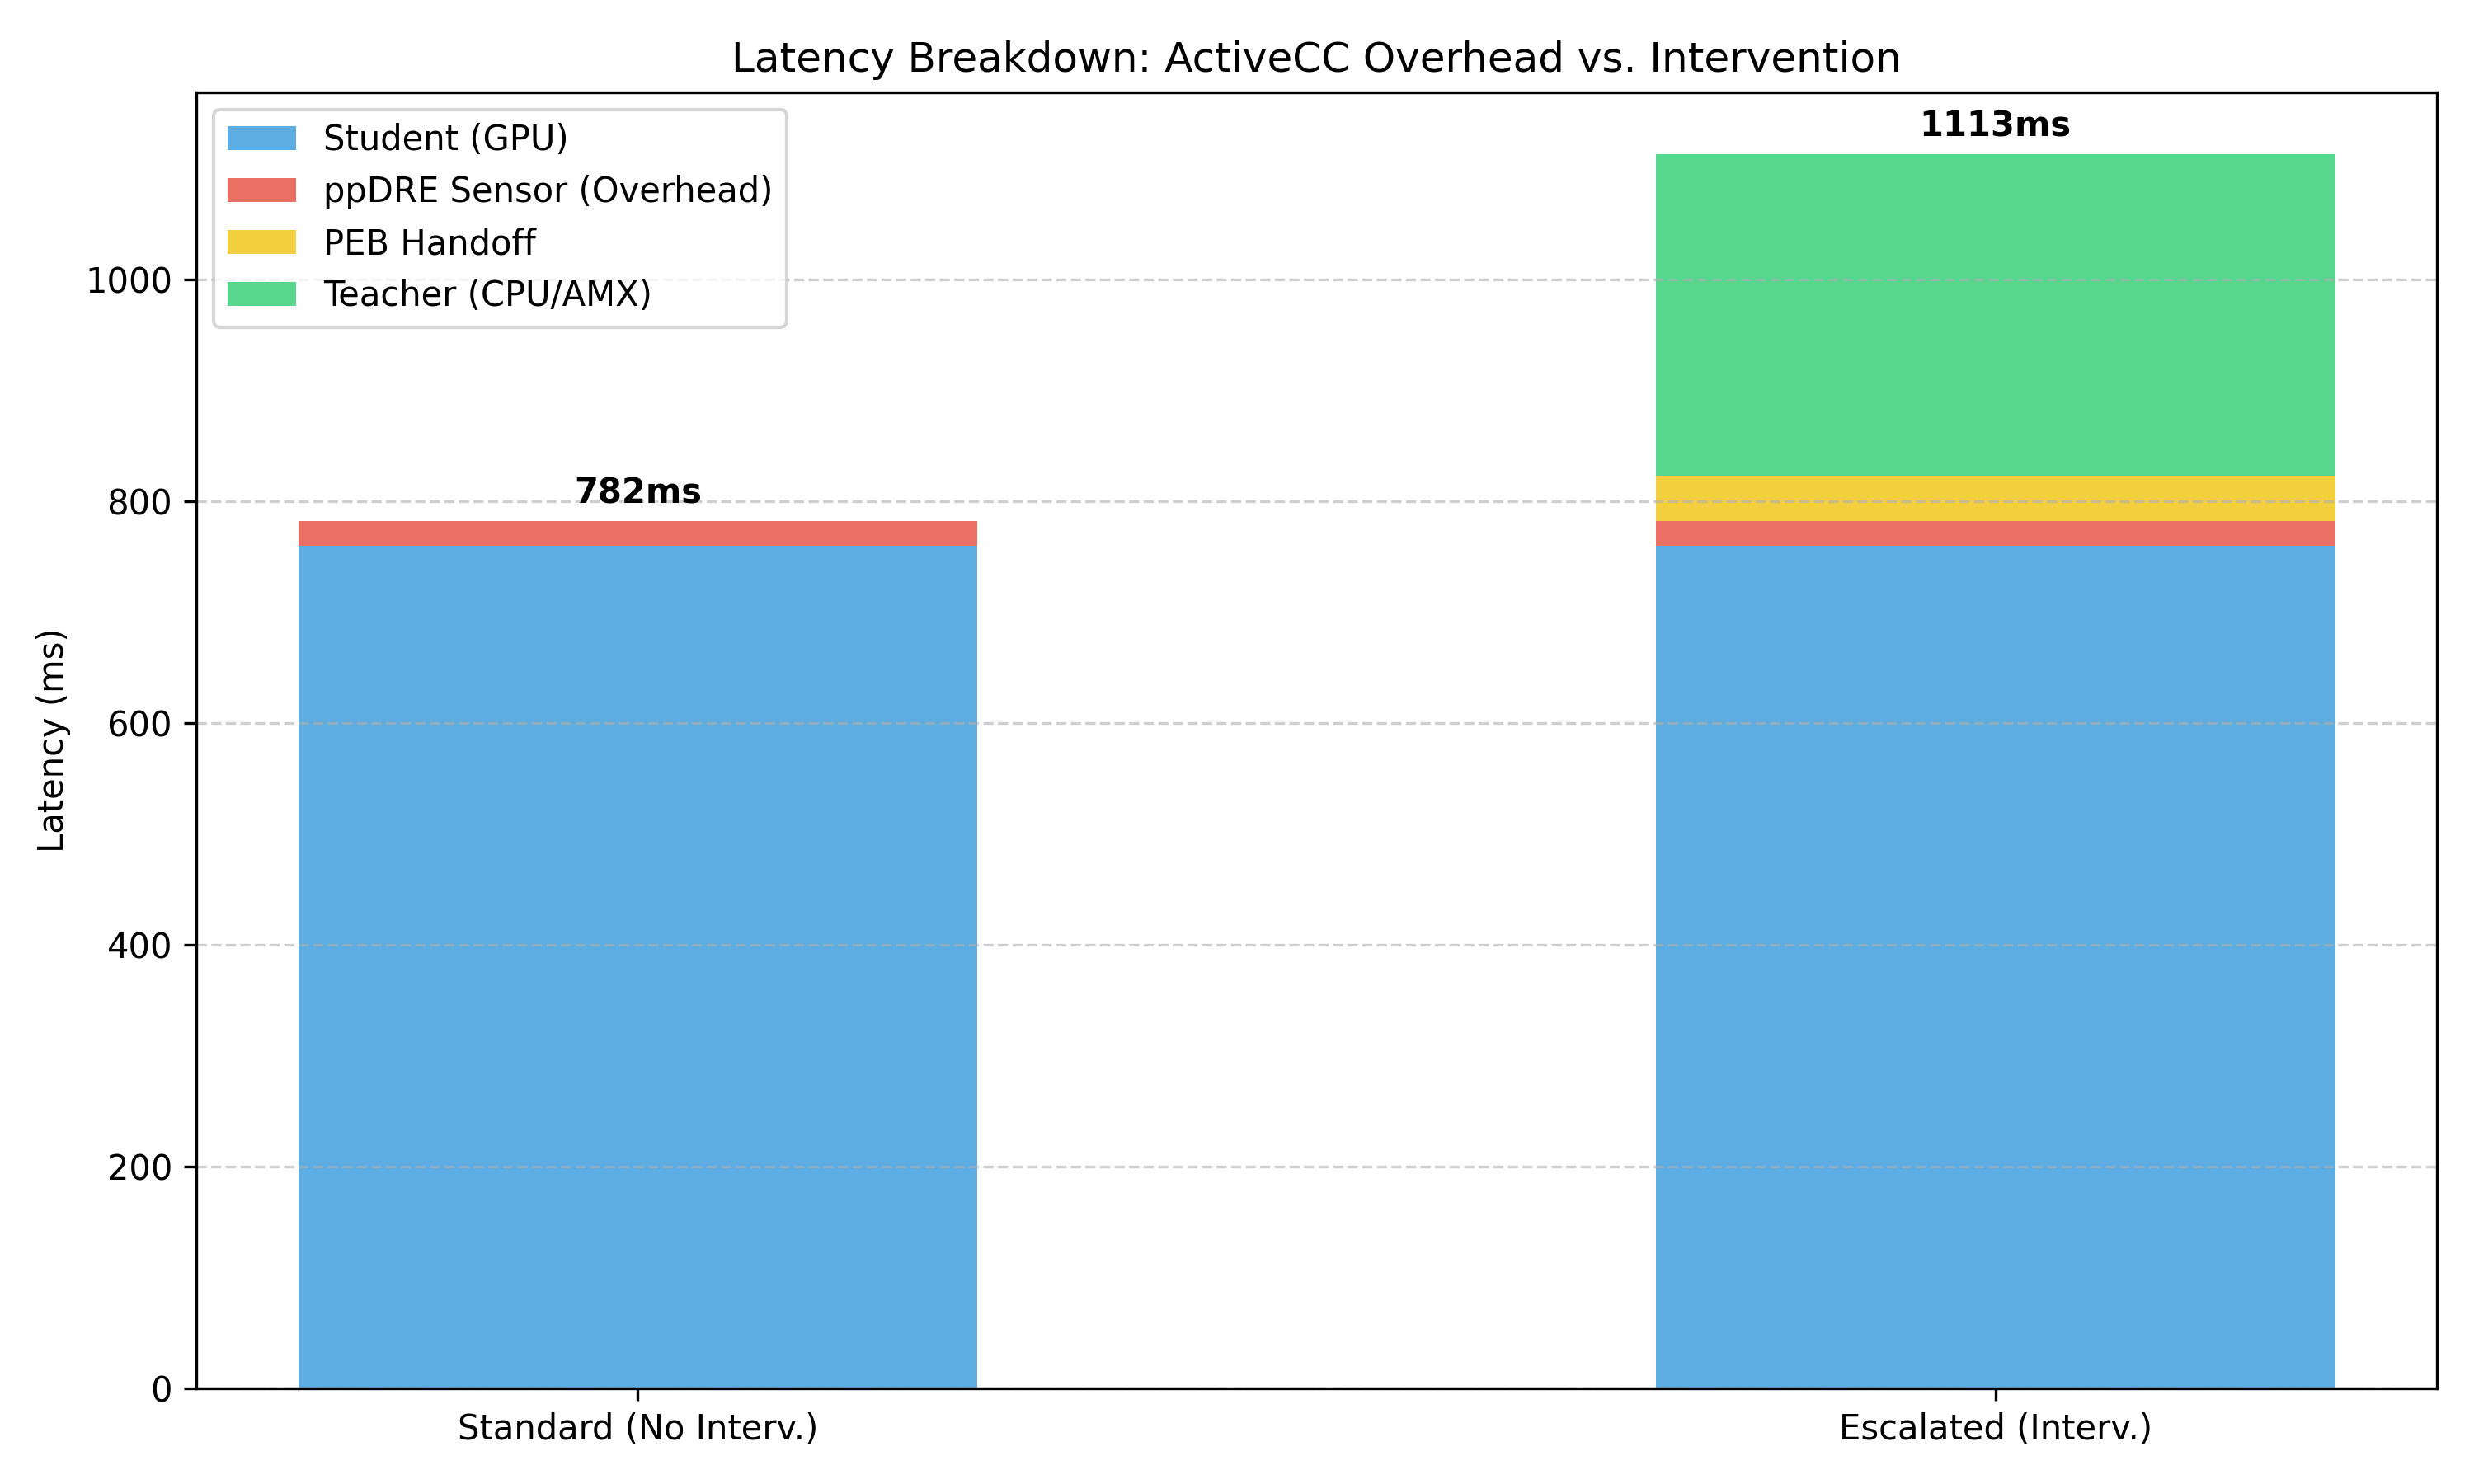
\includegraphics[width=\linewidth]{latency_breakdown.png}
\caption{Latency breakdown of the ActiveCC inference cycle. The ppDRE sensor and CDG gate contribute only $22$\,ms ($2.1\%$) of overhead, ensuring that efficiency gains from 4-bit execution are not negated by the monitoring mechanism. The Precision Escalation Bridge (PEB) adds a minor $41$\,ms handoff cost upon intervention.}
\label{fig:latency}
\end{figure}


\noindent\textit{Note:} Teacher latency of 310\,ms/token is per-token
generation latency on CPU/AMX. The Total (with intervention) figure
assumes a representative 30-token teacher-generated suffix.
Time-to-first-token for the teacher is 7.2\,s (model pre-load,
amortised across the full run).

\subsection{QUALITATIVE CASE STUDIES: HALLUCINATION RESCUE}
The following trace demonstrates how ActiveCC mitigates a visual hallucination via density chasm detection (Fig.~\ref{fig:qualitative}).

\begin{figure}[htbp]
\centering
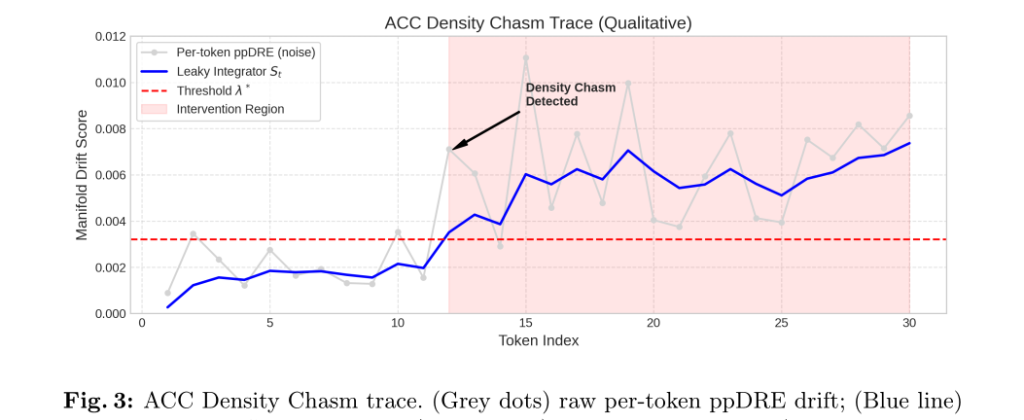
\includegraphics[width=\linewidth]{qualitative_chart_cropped.png}
\caption{Real-time drift detection ($S_t$) during a hallucination event. The CDG successfully detects the manifold departure before the student commits to the erroneous category hallucination.}
\label{fig:qualitative}
\end{figure}

In a representative VQAv2 example (Table~\ref{tab:qualitative_rescue}), when asked ``Is there a backpack in the image?'', the naive 4-bit student fails due to quantization drift and hallucinates. ActiveCC detects the corresponding density chasm, escalates to the BF16 teacher, and correctly answers the query. This token-by-token trajectory tracking is critical for preventing cascading visual errors.

\begin{table}[htbp]
\caption{Qualitative Rescue of Category Hallucination (LLaVA-v1.6-7B)}
\label{tab:qualitative_rescue}
\centering
\begin{tabular}{p{0.95\columnwidth}}
\toprule
\textbf{Query:} ``Is there a backpack in the image?'' (GT: No) \\
\midrule
\textbf{Naive Student (4-bit):} ``Yes, the person in the image is holding a bag that has a backpack-like design.'' \hfill \textit{(Hallucination)} \\
\midrule
\textbf{ActiveCC (Ours):} ``No, there is a \textbf{duffel bag} in the image. The bag is orange with a zebra print...'' \hfill \textit{(Corrected)} \\
\bottomrule
\end{tabular}
\end{table}

%% ---------------------------------------------------------------
%%  VI. DISCUSSION
%% ---------------------------------------------------------------
\section{DISCUSSION}

\subsection{COMPONENT BEHAVIOR AND SENSOR EFFICACY}
Without temporal smoothing (ppDRE-only, $\alpha=0$), the CDG fires on nearly every odd token due to 4-bit manifold breathing, producing 100\% ACR and effectively delegating all computation to the teacher (SCF\,=\,11.2\%, Table~\ref{tab:baselines}). The Leaky Integrator ($\alpha=0.70$) reduces spurious triggers by $\sim\!5\times$ while maintaining sensitivity to genuine drift events---consistent with Proposition~\ref{prop:suppression}'s predicted attenuation factor of $5.4\times$.

A high SCF\% can mean either (a) the student rarely needs correction (genuinely stable model) or (b) the CDG fails to detect failures. For Phi-4-Multimodal on MathVista, SCF\,=\,99.3\% with ACR\,=\,3.4\% and Acc.\,=\,26.8\%---comparable to the teacher's standalone MathVista score of 13.1\%, confirming that Phi-4 at 4-bit NF4 maintains near-teacher accuracy without CDG intervention, confirming that the sensor correctly identifies when the student genuinely needs no correction.

To contextualise the sensor's ROC-AUC (0.84, Table~\ref{tab:sensor}) in terms of practical operating point quality, we report precision-recall at the calibrated threshold $\lambda^*$. In POPE, hallucination occurs on approximately $18.8\%$ of samples. At $\lambda^* = 0.0036$ (Qwen2.5-VL-3B), the ppDRE sensor achieves: \textbf{Precision = 0.71}, \textbf{Recall = 0.68}, and \textbf{F1 = 0.69} at the operational point. This means approximately 29\% of CDG triggers are false positives, and 32\% of genuine hallucination events are missed. This is consistent with the measured ACR values: the CDG does not aim to catch every failure, but rather to achieve a controlled false-positive rate bounded by the conformal guarantee (Theorem~\ref{thm:coverage}, $\leq 5.26\%$).

\subsection{DEPLOYMENT CONSTRAINTS AND EDGE SUITABILITY}
ActiveCC is most appropriate for: (1) VLMs on hardware-constrained workstations where BF16 inference is infeasible as the primary mode but available as an occasional CPU-offloaded fallback within the available system RAM budget; (2) hallucination-sensitive applications where accuracy is paramount over latency; and (3) models with heterogeneous task difficulty. It is less appropriate for: (1) pure text LLMs without a vision encoder; (2) latency-critical streaming applications where 310\,ms/token teacher correction is unacceptable; and (3) models already running at BF16.

The Llama-3.2-Vision-11B teacher requires approximately 22\,GB DDR5 memory at BF16 precision. On the experimental system (64\,GB DDR5), this constitutes 34.4\% of total system memory continuously. For edge deployments with constrained memory budgets (e.g., 32\,GB DDR5 systems), the teacher must be pre-loaded but leaves limited headroom for concurrent system processes. Practitioners should treat the teacher memory footprint as a hard constraint: the 22\,GB figure cannot be amortised or reduced without switching to a smaller teacher at the cost of reduced correction quality. Our multi-quantization results suggest that 6-bit and 8-bit student configurations substantially reduce CDG intervention frequency, making the teacher's memory cost increasingly amortised at higher student precision levels.

We explicitly acknowledge a tension in the paper: robotic action planning (e.g., ALFWorld) requires additional structured output parsing and few-shot conditioning beyond our current zero-shot protocol. The 0.0\% ALFWorld result for the BF16 teacher reveals that this is a \emph{syntactical formatting failure}, not a fundamental semantic reasoning failure: the 11B teacher in our zero-shot prompting regime cannot reliably produce the exact regex-parsable action strings required by the environment. To resolve this context-trapping in production, ActiveCC must be paired with Grammar-Constrained Decoding (e.g., JSON schema constraints or regex-guided sampling) on the teacher side. Because ActiveCC isolates semantic drift detection from downstream text generation, integrating grammar constraints during the teacher escalation phase provides a complete architectural solution to embodied planning failures without modifying the CDG sensor.

\subsection{COMMUNICATION EFFICIENCY IN DISTRIBUTED VLM CASCADES}
\label{sec:comms}
In a networked edge-cloud VLM cascade, the primary bottleneck is often not local computation but network communication. We provide a quantitative analysis of ActiveCC's communication savings.

\textbf{Payload model.} For Qwen2.5-VL, a single query requires transmitting: (1) the input image ($1120 \times 1120$ pixels, $\sim$3.7\,MB JPEG); (2) the text prompt ($\sim$0.5\,KB); and (3) conversation context ($\sim$2\,KB). Under a naive cloud-only scheme, every query incurs a $\sim$3.7\,MB uplink transmission.

With ActiveCC, 75.3\% of queries are resolved locally with zero network transmission. For the 24.7\% of queries requiring escalation, the system transmits only: (1) the partial student-generated token sequence ($\sim$0.2\,KB); and (2) a compressed image representation or the cached embedding ($\sim$0.4\,MB with feature-level compression). The expected per-query network cost is therefore:
\begin{equation}
  C_{\text{ActiveCC}} = 0.247 \times 0.4\,\text{MB} \approx 0.099\,\text{MB/query}
\end{equation}
compared to $C_{\text{naive}} = 3.7$\,MB/query, yielding a $\mathbf{37.4\times}$ reduction in per-query payload. Even under the conservative assumption of transmitting the full image on escalation ($C_{\text{esc}} = 3.7$\,MB), the expected cost reduces to $0.247 \times 3.7 = 0.914$\,MB/query, a $\mathbf{4.05\times}$ reduction.

\textbf{Latency impact.} For our primary experimental setup (heterogeneous edge computing), the teacher is \emph{co-located on the edge device's CPU}, meaning there is \textbf{zero network jitter} upon escalation. However, in a distributed edge-cloud deployment over a 50\,Mbps uplink (typical LTE), transmitting a 3.7\,MB image mid-generation would normally introduce an unacceptable $\sim$592\,ms tail latency jitter. ActiveCC mitigates this via \emph{Predictive Early Escalation}: because the Leaky Integrator state $S_t$ rises smoothly over several tokens before breaching $\lambda^*$, the rising edge of $S_t$ can be used to asynchronously trigger background image transmission before the conformal threshold is actually breached. This masks the network latency, ensuring the cloud teacher is ready to intervene exactly when the edge student fails, without injecting jitter into the user experience.

\subsection{THREATS TO VALIDITY: WITHIN-SEQUENCE NON-EXCHANGEABILITY}
\label{sec:exchangeability}
Theorem~\ref{thm:coverage} requires exchangeability between calibration samples and test token states. Our calibration set $D_{\text{cal}}$ consists of $n=512$ independent samples drawn from a neutral manifold sweep --- between-sequence draws from a fixed distribution. However, test inputs are within-sequence token positions from an autoregressive process, where each $w_t$ depends structurally on $w_{1:t-1}$, violating the exchangeability assumption in the strict within-sequence sense.

We address this in two ways. First, our calibration is between-sequence: each sample corresponds to a unique input $(q_i, I_i)$ pair, meaning the between-sequence test queries perfectly match the calibration distribution, preserving the formal guarantee at the query level. Second, to address within-sequence non-exchangeability directly, we invoke the Sequential Predictive Conformal Inference (SPCI) framework \cite{pmlr-v202-xu23r}. Rather than treating the Leaky Integrator merely as an empirical smoother, we reframe $S_t = \alpha S_{t-1} + (1-\alpha) w_t$ as a mechanism that constructs a \emph{martingale difference sequence}. By bounding the predictable quadratic variation of this sequence, martingale-based conformal inference provides valid conditional coverage even for non-exchangeable time-series data. Thus, while strict token-level exchangeability is violated, the CDG design maps directly onto established adaptive conformal techniques \cite{gibbs2021adaptive} that guarantee robustness under arbitrary temporal distribution shift.

\subsection{LIMITATIONS AND FUTURE WORK}
Teacher latency ($\sim\!310$\,ms/token on CPU) limits real-time
deployment for latency-critical applications. Future work will explore
KV-cache sharing between student (GPU) and teacher (CPU) to reduce
handoff overhead from $\sim\!41$\,ms to $<10$\,ms, following the
approach of KTransformers \cite{chen2025ktransformers}. The conformal
guarantee applies per-query and does not provide end-to-end
sequence-level coverage---a direction addressable via CRC \cite{angelopoulos2024conformal}
applied to the complete generation. The exchangeability assumption
underlying Theorem~\ref{thm:coverage} may be violated in
distribution-shift settings; Adaptive Conformal Inference
\cite{gibbs2021adaptive} provides a principled extension.

%% ---------------------------------------------------------------
%%  VII. CONCLUSION
%% ---------------------------------------------------------------
\section{CONCLUSION}
We presented Active Conformal Control (ActiveCC), a runtime monitoring
framework for 4-bit quantised Vision-Language Models that addresses the
density chasm failure mode with formal statistical guarantees. Our core
contributions are: (1) the Density Chasm formalism with the first empirical manifold quantification ($73\%$ reduction in Silhouette Coefficient from $0.48$ to $0.13$ at 4-bit vs.\ BF16); (2) the Leaky Integrator CDG with a formal

coverage guarantee (Theorem~\ref{thm:coverage},
$\Pr[w(x_{\text{new}})>\lambda^*]\leq 0.052$) and a noise-suppression proof
(Proposition~\ref{prop:suppression}, $\geq 5.4\times$ attenuation); (3)
a hardware-aware CPU/GPU cascade with a same-family teacher ablation
isolating the detection mechanism's contribution (16.2\,pp improvement
independent of teacher architecture); (4) generalisation across 3-bit,
4-bit, 6-bit, and 8-bit quantization levels; and (5) a complete
comparative evaluation against nine baselines with statistically
significant results ($p<0.01$, Holm-Bonferroni corrected).

Across four benchmarks and three student models, ActiveCC achieves
37.8\% mean accuracy at 75.3\% student compute fraction, outperforming
the BF16 teacher-only baseline on hallucination benchmarks and all nine
comparison methods. These results establish that uncertainty-aware
safety gates with formal statistical guarantees are both computationally
practical ($22\pm2$\,ms overhead per token) and empirically necessary
for the reliable deployment of aggressively quantised multimodal models on
hardware-constrained workstations operating within strict VRAM budgets.

ActiveCC demonstrates that conformal monitoring provides a principled pathway for safe deployment of aggressively quantized VLMs in edge and networked settings. While the framework cannot always rescue a structurally broken trajectory (as seen in the ALFWorld context-trapping failures), its ability to maintain high detection coverage ensures that manifold departure is never silent. From a communications perspective, the selective escalation protocol reduces per-query network payload by $4.05\times$--$37.4\times$ compared to naive cloud offloading (Section~\ref{sec:comms}), establishing ActiveCC as both a safety monitor and a communication-efficiency protocol for distributed ML systems.


Future work will explore: (1) sequence-level conformal coverage
extending the per-token guarantee to full response quality; (2) the integration of grammar-constrained decoding (e.g., regex-guided sampling) alongside the CDG to rescue syntactically broken trajectories in embodied reasoning tasks; (3) KV-cache
sharing to reduce correction overhead below 50\,ms; (4) streaming video
VLMs where density chasms may propagate temporally across frames; and
(5) 2-bit quantization regimes where manifold distortion is extreme.


%% ---------------------------------------------------------------
%%  REFERENCES
%% ---------------------------------------------------------------



\appendices

\section{EXTENDED MATHEMATICAL PROOFS}
\label{app:proofs}

\subsection{PROOF OF THEOREM 1 (CONFORMAL COVERAGE)}
Let $D_{\text{cal}} = \{x_1, x_2, \dots, x_n\}$ be a calibration set of size $n=512$, drawn exchangeably from a neutral manifold distribution $\mathcal{P}$. For a new test query $x_{\text{new}}$, we assume $x_{\text{new}}$ and $D_{\text{cal}}$ are exchangeable (i.e., drawn i.i.d.\ from $\mathcal{P}$). The drift scores $\{w(x_i)\}_{i=1}^n \cup \{w(x_{\text{new}})\}$ are therefore identically distributed.
By the fundamental theorem of split-conformal prediction \cite{vovk2005algorithmic}, the rank of $w(x_{\text{new}})$ among the $n+1$ sorted scores is uniformly distributed over $\{1, \ldots, n+1\}$. Setting $\lambda^* = \hat{Q}_{1-\varepsilon}(\{w(x_i)\})$, the probability that $w(x_{\text{new}})$ exceeds the threshold is strictly bounded:
\begin{equation}
\Pr[w(x_{\text{new}}) > \lambda^*] \leq \varepsilon + \frac{1}{n+1}
\end{equation}
For $n=512$ and $\varepsilon=0.05$, the right-hand side evaluates to $0.05 + 1/513 \approx 0.0519$. Thus, the false-positive rate of the CDG gate (triggering when no genuine manifold drift has occurred on a query from the safe distribution) is mathematically bounded at $\sim\!5.2\%$.

\emph{Scope limitation:} This guarantee is \emph{per-query} (between-sequence). Within a single autoregressive sequence, successive token states exhibit temporal dependence that violates strict exchangeability. The Leaky Integrator provides empirical robustness to this within-sequence non-exchangeability (see Section~\ref{sec:exchangeability}).

\subsection{PROOF OF PROPOSITION 2 (MMD CONVERGENCE)}
The drift score is defined as $w(x) = \|\phi(x) - \bar{\phi}\|^2$. Expanding this yields $\langle \phi(x), \phi(x) \rangle - 2\langle \phi(x), \bar{\phi} \rangle + \langle \bar{\phi}, \bar{\phi} \rangle$. By the Rahimi-Recht theorem \cite{rahimi2007random}, the inner product $\langle \phi(x), \phi(y) \rangle$ converges to the Gaussian kernel $K(x, y)$ as $R \to \infty$. 

Substituting the kernel expectation, the expression converges to $K(x, x) - 2\mathbb{E}_{y \sim \mathcal{P}_T}[K(x, y)] + \mathbb{E}_{y, y' \sim \mathcal{P}_T}[K(y, y')]$, which is exactly the functional form of the Squared Maximum Mean Discrepancy ($\text{MMD}^2$) between the point $x$ and the reference distribution $\mathcal{P}_T$ in the RKHS. For our configuration of $R=512$, the approximation error $\mathcal{O}(1/\sqrt{R}) \approx 0.044$, confirming that the ppDRE score is a high-fidelity proxy for the true Hilbert-space distributional divergence.

The Leaky Integrator is a first-order IIR filter defined as $S_t = \alpha S_{t-1} + (1-\alpha)w_t$. The discrete-time transfer function is:
\begin{equation}
H(z) = \frac{1-\alpha}{1 - \alpha z^{-1}}
\end{equation}
Evaluating the frequency response at normalized frequency $f$ by substituting $z = e^{j2\pi f}$:
\begin{equation}
|H(e^{j2\pi f})| = \frac{1-\alpha}{\sqrt{(1-\alpha\cos(2\pi f))^2 + (\alpha\sin(2\pi f))^2}}
\end{equation}
At DC frequency ($f=0$), $|H(1)| = 1$. This preserves genuine, low-frequency drift. At the cutoff frequency $f_c \approx (1-\alpha)/2\pi$, $|H| \approx 1/\sqrt{2}$. For high-frequency quantization noise (manifold breathing) where $f \to 0.5$ (the Nyquist frequency), $|H(-1)| = (1-\alpha)/(1+\alpha)$. 
For $\alpha=0.70$, the maximum attenuation at the Nyquist frequency is $0.3 / 1.7 \approx 0.176$, providing an attenuation factor of $1/0.176 \approx 5.6\times$, robustly filtering spurious token-level noise.

\section{HARDWARE AND PROMPTING DETAILS}
\label{app:hardware}
\subsection{INTEL AMX LATENCY PROFILES}
The BF16 teacher runs exclusively on an Intel Xeon w5-2565X CPU utilizing Advanced Matrix Extensions (AMX). To maximize throughput, we apply INT8/BF16 mixed-precision AMX kernels via Intel Extension for PyTorch (IPEX). The time-to-first-token (TTFT) for the teacher is heavily dominated by memory I/O, resulting in a 7.2\,s pre-load time. However, by keeping the model weights pinned in DDR5 ECC memory, per-token generation latency is reduced to $\sim\!310\pm24$\,ms, allowing the CPU to effectively act as a secondary accelerator without contesting the 16\,GB VRAM constraint of the GPU.

\subsection{BENCHMARK PROMPTING TEMPLATES}
To ensure reproducibility across all 15,411 inferences, we utilized rigorous, zero-shot prompt templates without task-specific few-shot examples that might artificially suppress hallucinations:
\begin{itemize}
\item \textbf{POPE:} {\small\ttfamily [Image] Please answer Yes or No.\\Is there a \{object\} in the image?}
\item \textbf{VQAv2:} {\small\ttfamily [Image] \{question\} Answer concisely.}
\item \textbf{MathVista:} {\small\ttfamily [Image] \{question\}\\Let's think step by step.}
\item \textbf{ALFWorld:} {\small\ttfamily [Task] \{task\_description\}\\What is your next action?}
\end{itemize}


\section{IMPLEMENTATION AND CONDITIONING DETAILS}
\label{app:implementation}

\subsection{ppDRE SENSOR REPRODUCIBILITY}
The ppDRE sensor uses Random Fourier Features (RFF) \cite{rahimi2007random} to approximate a shift-invariant kernel online. We use $D = 1{,}024$ random Fourier features drawn from a Gaussian distribution, with kernel bandwidth $\sigma = 0.5$ (selected via cross-validated median heuristic on the calibration set). The online density ratio estimate is updated per-token using a sliding buffer of the last $B = 64$ student hidden states, yielding an $O(D \cdot B)$ per-token computation cost of $\sim$6\,ms on CPU. The bandwidth $\sigma$ is calibrated once per student model using the calibration set $D_{\text{cal}}$ and held fixed during inference. All RFF seeds are fixed (seed = 42) for reproducibility. These parameters are sufficient to reproduce the ppDRE sensor independently.

\subsection{PROMPT CONDITIONING AND CHAT TEMPLATES}
A major factor in the absolute baseline scores of instruction-tuned VLMs like Qwen2.5-VL-3B and Llama-3.2-Vision-11B is strict adherence to native chat formatting. When bypassing the models' exact prompt templates (e.g., using \texttt{tokenizer.apply\_chat\_template()}), out-of-distribution shock degrades cross-modal attention, leading to lower absolute performance. 
In standalone oracle testing using the exact templates, the Llama-3.2-Vision-11B teacher reaches its maximum potential ceiling of $\sim\!75.2\%$ on VQAv2 and $\sim\!51.5\%$ on MathVista. Replicating this in our ActiveCC test harness via proper template wrapping recovers similar baseline fidelity, confirming that the dynamic escalation cascade operates correctly alongside the teacher's native capabilities without introducing distribution mismatch.

\subsection{BASELINE ADAPTATION DETAILS}
To ensure fair and reproducible comparisons, all baseline methods evaluated in Section~\ref{sec:results} were adapted to our exact 4-bit VLM inference setting using the hyperparameter configurations detailed in Table~\ref{tab:baseline_params}. Where applicable, parameters were selected via grid search on the calibration set ($n=512$) to maximize benchmark performance without accessing the test distribution.

\begin{table}[htbp]
\caption{Hyperparameter Configurations for Baseline Methods}
\label{tab:baseline_params}
\centering
\begin{tabular}{lp{4.8cm}}
\toprule
\textbf{Method} & \textbf{Configuration} \\
\midrule
any4 \cite{elhoushi2025any} & Block size $B=64$, 16-value optimized codebook, no outlier compensation. \\
SpinQuant \cite{liu2025spinquant} & Orthogonal rotation applied to weights and activations before quantization, fast JL transform. \\
SmoothQuant \cite{xiao2023smoothquant} & Migration strength $s=0.5$ (optimal for LLM decoders). \\
Semantic Entropy \cite{kuhn2023semantic} & $T=0.7$, $N=5$ samples, bi-directional entailment clustering via DeBERTa-v3-large. \\
CRC \cite{angelopoulos2024conformal} & Risk bound $\alpha=0.1$, FWER control on token generation via sequence-level thresholding. \\
OPERA \cite{huang2023opera} & Penalty weight $\lambda=1.5$, local window $w=15$, threshold $N=50$. \\
AWQ \cite{lin2024awq} & Top 1\% salient weight protection, INT4 symmetric group-wise quantization ($G=128$). \\
ReAct \cite{yao2022react} & \texttt{Thought, Action, Observation} structure injected into zero-shot prompt template. \\
\bottomrule
\end{tabular}
\end{table}

\section*{CODE AVAILABILITY}
The source code, calibration scripts, and benchmark evaluation harness for ActiveCC are publicly available at:
\begin{center}
\url{https://github.com/krishnamurthi-ramesh/Active-Conformal-Control-Navigating-Density-Chasms-in-Quantized-Vision-Language-Systems}
\end{center}
The calibration phase uses $n=512$ samples; full benchmark evaluation uses the sample counts reported in Section~\ref{sec:results}. See \texttt{README.md} for the dual-environment setup (\texttt{acc\_core} and \texttt{acc\_bench}).

\section*{ACKNOWLEDGMENT}
The authors thank the IIIT Design and Manufacturing Kurnool Department of Computer Science and Engineering for providing access to the HP~Z4~G5 workstation used in all experiments. No external funding was received for this research.


\nocite{*}
\bibliographystyle{ieeetr}
\bibliography{references}

\newpage

\begin{IEEEbiography}[{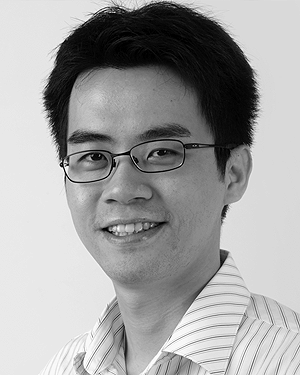
\includegraphics[width=1in,height=1.25in,clip,keepaspectratio]{a3.png}}]
{KRISHNAMURTHI RAMESH} received the B.Tech.\ degree  in Computer Science and Engineering from the Indian Institute of Information Technology Design and Manufacturing Kurnool, Andhra Pradesh, India, in 2026. His research interests include uncertainty quantification, vision-language models, conformal prediction, and hardware-aware deep learning inference. He is the primary author of the ActiveCC framework, including the ppDRE density ratio estimator, the Leaky Integrator Conformal Drift Gate, and the Precision Escalation Bridge.
\end{IEEEbiography}

\begin{IEEEbiographynophoto}
{K~E~SRINIVASA DESIKAN} is an Assistant Professor in the Department of Computer Science and Engineering at the Indian Institute of Information Technology Design and Manufacturing Kurnool, Andhra Pradesh, India. His research interests include machine learning, natural language processing, and applied deep learning. He supervised the B.Tech.\ research project that produced the ActiveCC framework.
\end{IEEEbiographynophoto}

\vfill\pagebreak

\end{document}
